
\newcommand{\nomedoc}{Piano Di Qualifica}
\newcommand{\versione}{2.1}
\newcommand{\versioneglossario}{2.0}
\newcommand{\versionenormeprogetto}{2.0}
\newcommand{\versioneAR}{3.0}
\newcommand{\versioneST}{2.0}
\newcommand{\nomefile}{PianoDiQualifica-\versione.pdf}
\newcommand{\datacreazione}{3 Dicembre 2010}
\newcommand{\datamodifica}{1 Febbraio 2011}
\newcommand{\stato}{formale}
\newcommand{\uso}{esterno}
\newcommand{\redazione}{Trezzi Giovanni}
\newcommand{\verifica}{Palazzin Alberto}
\newcommand{\approvazione}{Lovato Daniele}
\newcommand{\distribuzione}{ 
VT.G \\
& Prof. Vardanega Tullio\\
& Prof. Cardin Riccardo }

% FUNZIONI TIPOGRAFICHE
\newcommand{\co}{\texttt} % courier
\newcommand{\bo}{\textbf} % bold
\newcommand{\pr}{\par\medskip} % paragrafo spaziato
\newcommand{\sca}{\textsc} % small caps

\documentclass[a4paper,12pt]{report}
% 10pt,11pt,12pt
% titlepage, notitlepage -> per dare inizio o no ad una nuova pagina dopo titolo
% twoside -> per dire se fronte-retro
\usepackage[latin1]{inputenc}
% per caratteri accentati
\usepackage[italian]{babel}
% per regole sintattiche italiane
\usepackage[bookmarks=true, pdfborder={0 0 0 0}]{hyperref}
% per collegamenti ipertestuali
\usepackage{graphicx}
% per inserimento immagini

% \usepackage{enumerate}
% per personalizzare elenchi puntati

\usepackage[hmargin=2cm]{geometry} %margine 2 cm
%\geometry{options varie}

% comandi per gestire meglio header e footer
\usepackage{fancyhdr}  % header e footer
\usepackage{totpages}
\pagestyle{fancy}
\renewcommand{\headrulewidth}{0.4pt}
\renewcommand{\footrulewidth}{0.4pt}

\setlength{\headheight}{1.2cm} % NON TOCCARE
\setlength{\voffset}{-1.5cm} % NON TOCCARE
\setlength{\textheight}{666pt} % NON TOCCARE
\setlength{\footskip}{60pt}
\setlength{\parindent}{0pt} % INDENTAZIONE

\lhead{\nomedoc\  (ver. \versione)}
\chead{}
\rhead{
\includegraphics[height=1cm]{img/netmus.png}}
\lfoot{
\includegraphics[height=0.8cm]{img/logo.png}}
\cfoot{}
\rfoot{\thepage}

\usepackage{titlesec}
\titleformat{\chapter}{\normalfont\huge\bfseries}
{\thechapter}{20pt}{\Huge}

\usepackage{rotating}   % PER TABELLE E AMBIENTI RUOTATI
\usepackage{array}
\usepackage{color}
\usepackage{colortbl}  % VARIE PER GESTIRE I COLORI
\definecolor{Orange}{RGB}{255,127,0}   % ARANCIO ACCES0
\definecolor{orange}{RGB}{255,207,80}  % ARANCIO TENUE

\addtocontents{toc}{\protect\thispagestyle{fancy}}  % PER INDICI CON + PAGINE
\usepackage[font=it]{caption}    % PER RENDERE CORSIVE LE DIDASCALIE
\usepackage{eurosym}  % PER SIMBOLO EURO

% \usepackage{listings}   per codice sorgente

\author{VT.G - Valter Texas Group}

\begin{document}

\pagenumbering{Roman} % INIZIO NUMERAZIONE ARABA

\vspace*{1cm}
\begin{center}

\begin{LARGE} \sca{Federico Baron} \end{LARGE}\\
\vspace{0.5cm}
\begin{Large}
\emph{fede.baron.89@gmail.com} \end{Large}\\
\vspace*{1cm} 
\includegraphics[width=5cm]{img/logo.png}\\
\vspace{0.5cm}
\begin{Large} \emph{``Comunicazione Aumentata/Alternativa per Giovani Ospiti
della Terapia Intensiva Pediatrica''} \end{Large}\\
\vspace{3cm}
\begin{Large} \sca{\nomedoc} \end{Large}\\
\end{center}
\vspace{1cm}

% INFORMAZIONI DOCUMENTO
\begin{center}
\begin{tabular}{r|l}
\hline & \\
\bo{Nome} & \nomefile \\
\bo{Versione attuale} & \versione \\
\bo{Data creazione} & \datacreazione \\
\bo{Data ultima modifica} & \datamodifica \\
\bo{Redazione} & \redazione \\
& \\\hline
\end{tabular}
\end{center}
\newpage

\chapter*{Sommario}
\thispagestyle{fancy}
Nelle pagine del presente documento saranno descritte le modalit\`a di verifica
e validazione che si intendono adottare e che verranno utilizzate durante
l'intero ciclo di vita del progetto, a partire dalla stesura dell'intera
documentazione fino alle ultime fasi di collaudo del software prima della
consegna del prodotto finale. Il Piano di Qualifica rappresenta di fatto il
punto di riferimento in cui sono contenute le linee guida da seguire per tutte
le attivit\`a di verifica e validazione.

\newpage
% REGISTRO MODIFICHE
\section*{Registro delle modifiche}

\begin{longtable}{|p{0.13\textwidth}|c|p{0.2\textwidth}|p{0.46\textwidth}|}
\hline
\rowcolor{orange} \bo{Data} & \bo{Versione} & \bo{Autore} & \bo{Descrizione} \\
\hline
\endhead
\hline
\endfoot
05/02/2011 & 2.1 & Daminato Simone & Inseriti i test di integrazione.\\
01/02/2011 & 2.0 & Baron Federico & Validazione per consegna RP.\\
\hline
31/01/2011 & 1.20 & Caputo Cosimo & Verificato intero documento.\\
\hline
31/01/2011 & 1.19 & Mandolo Andrea & Inseriti Esiti di Verifica sulla
Progettazione ad Alto Livello. Corretti tutti gli errori segnalati.\\
\hline
\hline
31/01/2011 & 1.18 & Palazzin Alberto & Aggiunta sezione 4.4 ``Dettaglio
dell'esito nel test di valutazione sul processo di lavoro''.\\
\hline
31/01/2011 & 1.17 & Palazzin Alberto & Aggiunto paragrafo ``Soddisfacimento di
tutti i requisiti individuati'' in 4.2.2.\\
\hline
29/01/2011 & 1.16 & Lovato Daniele & Aggiunta Tabella Tracciamento requisiti e
metodi di verifica in fase di collaudo.\\
\hline
29/01/2011 & 1.15 & Palazzin Alberto & Tolto paragrafo ``Principi e linee
guida''.\\
\hline
29/01/2011 & 1.14 & Mandolo Andrea & Aggiunta la verifica dei requisiti di
analisi v.1.7 e indicati come modificati a fronte della precedente verifica
sulla versione 1.6.\\
\hline
28/01/2011 & 1.13 & Lovato Daniele & Sistemata Sezione 3.1 e 3.2.
Perfezionata sezione 5.1.\\
\hline
28/01/2011 & 1.12 & Palazzin Alberto & Correzione errori ortografici.
Sistemazione dei termini enfatizzati. Aggiunto strumento ASPELL. Correzione
semantica. Correzione della punteggiatura su elenchi puntati.
Ridimensionamento misure delle tabelle sui dettagli della verifica
dell'analisi. Eliminato sottoparagrafo 2.7.3 ``Verifica tramite test''.
Aggiunti i link per reperire gli strumenti. Aggiunto paragrafo 4.4 ``Dettaglio
dell'esito delle revisioni''.\\
\hline
27/01/2011 & 1.11 & Mandolo Andrea & Aggiunto lo Scheduling nei risultati
della verifica dell'analisi.\\
\hline
27/01/2011 & 1.10 & Trezzi Giovanni & Correzione errori grammaticali. Aggiunto
l'esito della verifica sulla qualit\`a dei requisiti. Paragrafo 4.2.1. Aggiunto
il risultato della verifica dei requisiti secondo il modello FURPS paragrafo
4.2.1. Aggiunto il sottoparagrafo ``Correttezza formale'' nei metodi di
verifica della documentazione.\\
\hline
26/01/2011 & 1.9 & Mandolo Andrea & Aggiunto
il paragrafo 2.7.1. ``Metodi di verifica per la documentazione'', aggiunta la
tabella ``Correzione documenti'' in Appendice. Aggiunto paragrafo 2.7.2 ``Metodi
di verifica per l'analisi'' e le tabelle B e C in appendice per la verifica dei requisiti.\\
\hline
26/01/2011 & 1.8 & Lovato Daniele & Aggiunta introduzione al paragrafo
``Analisi dinamica'' e corretto il contenuto nella sua forma. Aggiunta
sottosezione ``Test di sistema''.\\
\hline
25/01/2011 & 1.7 & Palazzin Alberto & Creato il paragrafo 3.3.1. Correzioni
grammaticali. Modifica del paragrafo 3.3.\\
\hline
25/01/2011 & 1.6 & Lovato Daniele & Modificata sezione ``Analisi dinamica''.\\
\hline
24/01/2011 & 1.5 & Palazzin Alberto & Aggiunta la tabella 2.1. Sistemato
l'indice del documento.\\
\hline
24/01/2011 & 1.4 & Lovato Daniele & Modificate le tecniche di analisi.
Modificato il paragrafo 2.1.3 e sistemato la verifica della fase progettuale.
Aggiunto paragrafo 2.9 ``Metodi di verifica''. Rimodulato il paragrafo 2.3
``Strumenti''. Aggiunti i metodi di verifica per la progettazione ad alto
livello, paragrafo 2.7.3.\\
\hline
23/01/2011 & 1.3 & Lovato Daniele & Spostato l'intero capitolo 4 alla fine
del capitolo 2, rinominato il capitolo 4 in ``Resoconto delle attivit\`a di
verifica'', rinominato il capitolo 5 in ``Pianificazione ed esecuzione del
collaudo''. Corretta forma e contenuto del capitolo 2 fino a 2.1.6 compreso,
spostato il paragrafo ``Metriche'' in 2.4.  
\\
\hline
21/01/2011 & 1.2 & Mandolo Andrea & Corretti Riferimenti.\\
\hline
12/01/2011 & 1.1 & Mandolo Andrea & Modificato layout Registro delle
modifiche.\\
\hline
19/12/2010 & 1.0 & Lovato Daniele & Validazione per consegna RR.\\
\hline
18/12/2010 & 0.6 & Palazzin Alberto & Verificato l'intero documento.\\
\hline
18/12/2010 & 0.5 & Trezzi Giovanni & Corretti errori di grammatica, sintattici
ed ortografici. Corretta la sintassi del paragrafo 3.2 del paragrafo 4.2 e
4.2.3.\\
\hline
13/12/2010 & 0.4 & Trezzi Giovanni & Corretti errori di battitura nel Sommario.
Modifiche sintattiche in 2.1. Scorporato 2.1.1 in 2.1.2, 2.1.3, 2.1.4. Modifica della
struttura di 2.1.2 in elenco puntato. Corretto errore grammaticale in 2.1.3.
Modifica sintattica in 2.1.4, in 2.2 e in 2.3.\\
\hline
3/12/2010 & 0.3 & Trezzi Giovanni & Corretto il contenuto del Sommario. Corretto
il paragrafo 1.2 ``Scopo del documento''. Modificato 2.1 integrando l'attivit\`a
di validazione nel discorso. Corrette le maiuscole/minuscole negli elenchi
puntati in 2.1.1, in 3.2 e 5. Corretto un errore di battitura in 3.3.1.
Modificato parte di 4.2 per maggior chiarezza di lettura.\\
\hline
13/12/2010 & 0.2 & Trezzi Giovanni & Correzione errori di battitura nei
paragrafi 2.1 3.1.2. Correzione punteggiatura degli elenchi puntati di tutto il documento.
Aggiunta la versione dei documenti a cui si fa riferimento.\\
\hline
03/12/2010 & 0.1 & Trezzi Giovanni & Stesura prima versione del documento.\\
\end{longtable}

% INDICE
\tableofcontents

\chapter{Introduzione}
\thispagestyle{fancy} % serve perche' nelle pagine di inizio Chapter esca header e footer
\pagenumbering{arabic} % INIZIO NUMERAZIONE NORMALE
\rfoot{\thepage\ di \pageref{TotPages}}

\section{Scopo del documento}

Il presente documento fornisce le strategie di \underline{verifica} e
\underline{validazione} che verranno attuate durante lo sviluppo del progetto al
fine di evitare ed eventualmente correggere anomalie e/o difetti all'interno del
sistema e per garantire l'insieme delle caratteristiche e propriet\`a che, nel
loro complesso, rappresentano la qualit\`a del prodotto finale.


\section{Scopo del prodotto}
Il progetto \underline{NetMus} nasce con lo scopo di realizzare un sistema
software basato su \underline{cloud} \underline{computing}, per memorizzare
informazioni di brani musicali in profili utente online.\\ Tali informazioni vengono estratte da
dispositivi musicali o di archiviazione \underline{USB} al momento della loro connessione.

\section{Glossario}
Il Glossario \`e definito con un documento a parte
(\emph{Glossario-\versioneglossario.pdf}). Tutti i termini caratterizzati da
\underline{questa sottolineatura} sono ivi definiti.\\
Verr\`a sottolineata solamente la prima occorrenza di ciascun
termine presente nel Glossario, per non compromettere la leggibilit\`a del documento.

\section{Riferimenti}

\subsection{Normativi} % oppure rif. a Norme di progetto con leggi e tutto
\begin{itemize}
  \item ISO/IEC 12207:1995 - Cicli di vita software
  \item ISO/IEC 9126:2001 - Quality Model
  \item \emph{NormeDiProgetto-\versionenormeprogetto.pdf} che regola e
  accompagna tutti i documenti ufficiali.
\end{itemize}
\newpage
\subsection{Informativi}
\begin{itemize}
  \item Capitolato d'appalto CO2-NETMUS del corso di Ingegneria del Software
  A.A. 2010/11 :\\
  \url{http://www.math.unipd.it/~tullio/IS-1/2010/Progetto/NetMus.pdf}
  \item Slide delle lezioni del corso:\\
  \url{http://www.math.unipd.it/~tullio/IS-1/2010/}
  \item Verbale intervista proponente:\\
  \co{allegato Verbale-1.0.pdf}
  \item Sistema di cloud Google App Engine:\\
  \url{http://code.google.com/intl/it/appengine/}
\end{itemize}


% INIZIO CAPITOLO 2

\chapter{Visione generale della \\strategia di verifica}
\thispagestyle{fancy} % serve perche' nelle pagine di inizio Chapter esca header e footer

\section{Organizzazione, pianificazione strategica e \\temporale,
responsabilit\`a}

Lo scopo che ci si prefigge \`e quello di garantire la pi\`u alta
\underline{qualit\`a} possibile per quello che sar\`a il prodotto finale. Con lo
scopo di garantire un'elevata qualit\`a, verranno stabilite precise procedure di
verifica su tutti i prodotti di ogni singola fase di lavoro, verranno indicati
gli strumenti con i quali effettuare le operazioni di verifica e verranno
indicate le strategie elaborate per poter operare in tal senso e ai fini di una
corretta validazione. Ogni singola modifica o l'insieme di pi\`u modifiche
comporteranno una conseguente attivit\`a di verifica. Al fine di
ottimizzare tempo e risorse, le attivit\`a verranno effettuate solamente quando
una singola o pi\`u modifiche avranno comportato differenze di tipo rilevante
all'interno di ogni fase del progetto. La validazione dovr\`a avvenire
solamente a fronte di una precisa e meticolosa attivit\`a di verifica e nel
rispetto di tutti i requisiti e le specifiche, senza discostarsi da
quanto inizialmente concordato. Sar\`a dovere del responsabile accertarsi che
tutte le attivit\`a si svolgano nelle modalit\`a descritte nel presente documento.
\\
\\ 
Come punto di riferimento per quanto riguarda la misurazione e quindi la
quantificazione della qualit\`a di ogni singolo processo nello sviluppo del
software faremo riferimento alla normativa ISO 15939 dove la misurazione del
software viene indicato come un processo iterativo PDCA, con 4 attivit\`a
principali.

\begin{figure}[h]
  \centering
  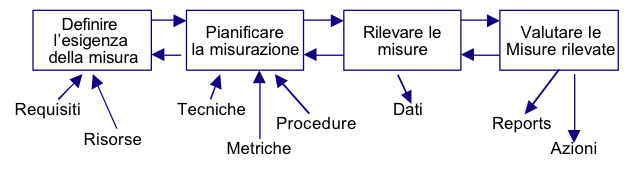
\includegraphics[height=4cm]{img/PQ/pdca.png}
\caption{Ciclo PDCA della misura}
\end{figure}

Nel presente capitolo verranno definite le esigenze di misurazione che si
ritengono necessarie ai fini della qualit\`a, ovvero verr\`a indicato cosa per ogni
singola fase del progetto sar\`a necessario verificare. Verranno indicati gli
strumenti con i quali effettuare la verifica e verranno indicate le metriche con
le quali misurare le propriet\`a di ci\`o che si sta verificando. Verranno
infine indicate le tecniche con le quali procedere. Una volta volta terminata
l'attivit\`a di verifica e la conseguente attivit\`a di misurazione, si proceder\`a con il
riportare l'esito nel capitolo 4 del presente documento. Dopodich\`e, terminata
l'attivit\`a di misurazione, sulla base dei risultati si valuteranno eventuali
decisioni, manovre correttive o l'accettazione del prodotto verificato secondo
le misure e i criteri stabiliti.


\subsection{Verifica della documentazione}

Per ogni documento dovranno essere verificati i seguenti aspetti:
\begin{itemize}
\item correttezza semantica e grammaticale;
\item chiarezza espositiva;
\item assenza di errori concettuali;
\item comprensibilit\`a e accuratezza;
\item correttezza e completezza dei concetti espressi;
\item formattazione del documento secondo quanto specificato dall'amministratore
in\\ \emph{NormeDiProgetto-\versionenormeprogetto.pdf}.
\end{itemize}

Nel caso sia necessario intervenire per correggere uno o pi\`u di questi aspetti
sar\`a dovere del verificatore contattare il redattore del documento affinch\'e
questo gestisca le relative attivit\`a di modifica. Una volta modificato, il
documento dovr\`a essere nuovamente sottoposto all'attenzione del verificatore
per una nuova attivit\`a di verifica.


\subsection{Verifica della fase di analisi}

La fase di analisi dovr\`a essere verificata secondo i seguenti aspetti:

\begin{itemize}

\item scheduling;
\item qualit\`a dei requisiti;
\item completezza del sistema definito rispetto al modello FURPS.
 

\end{itemize}

Il modello FURPS \`e stato elaborato inizialmente da Robert Grady presso i
laboratori dell'Hewlett-Packard. \`E un acronimo mnemonico per la definizione dei requisiti
di software di vario genere e sta a significare:

\begin{itemize}

\item F - Functionality (capacit\`a di fornire le funzioni richieste);
\item U - Usability (facilit\`a d'uso dell'utenza finale);
\item R - Reliability (gestione degli errori e dei crash);
\item P - Performance (Prestazioni);
\item S - Supportability (Supportabilit\`a).
\end{itemize}


Nel caso sia necessario intervenire in maniera correttiva rispetto ad uno o
pi\`u di questi aspetti sar\`a dovere del verificatore contattare l'analista
responsabile affinch\'e provveda alle relative modifiche.



\subsection{Verifica della fase progettuale}

La fase di progettazione dovr\`a essere verificata secondo i seguenti aspetti:

\begin{itemize}

\item soddisfacimento di tutti i requisiti individuati nel documento
\emph{AnalisiDeiRequisiti-\versioneAR.pdf};
\item individuazione di elementi progettuali superflui, non aderenti a nessun
requisito richiesto;
\item corretta corrispondenza e tracciabilit\`a tra i requisiti e le relative
parti del progetto;
\item flessibilit\`a;
\item manutenibilit\`a.

\end{itemize}

Nel caso sia necessario intervenire in maniera correttiva rispetto ad uno o
pi\`u di questi aspetti sar\`a dovere del verificatore contattare il progettista
responsabile affinch\'e provveda alle relative modifiche riguardanti la progettazione.

\subsection{Verifica della fase di realizzazione/programmazione}

La fase di realizzazione/programmazione dovr\`a essere verificata secondo i seguenti aspetti:
\begin{itemize}
\item corretto funzionamento dell'applicazione;
\item affidabilit\`a;
\item efficienza;
\item portabilit\`a;
\item manutenibilit\`a.

\end{itemize}

Nel caso sia necessario intervenire sul codice in base ad uno di questi aspetti
sar\`a dovere del verificatore contattare il programmatore responsabile della
relativa porzione di codice.

Inoltre, per favorire l'attivit\`a di verifica, ogni programmatore sar\`a tenuto
ad eseguire attivit\`a di rilevazione degli errori sul codice per cercare di
diminuire le possibilit\`a d'errore.

\subsection{Validazione}

L'impegno che ci si assume \`e quello di fornire un prodotto completamente e
correttamente funzionante secondo i requisiti concordati. Qualora venissero
riscontrati difetti o non conformit\`a, durante la verifica in fase di collaudo,
ci si impegna ad effettuare modifiche o interventi necessari per risolvere i
problemi.

\section{Risorse necessarie e disponibili}

Per la fase di qualifica sono necessarie risorse di tipo umano che
effettueranno attivit\`a di verifica e validazione cos\`i come definito nel
presente documento. Sono necessarie inoltre risorse di tipo logistico quali
programmi per le attivit\`a di tracciamento tra i requisiti e i moduli software,
un \underline{framework} per i test specifici di unit\`a del codice, un
applicativo software per la gestione e la risoluzione delle anomalie, un ambiente di sviluppo
adeguato con possibilit\`a per i programmatori di rilevare gli errori.


\section{Strumenti}

Per le attivit\`a di verifica ci avvarremo dei seguenti strumenti:

\begin{itemize}

\item Aspell: per controllo ortografico dei
documenti con estensione .tex, necessita di importare un dizionario italiano
(per informazioni \url{http://aspell.net/});

\item JUnit: come unit test framework per il linguaggio di
programmazione \underline{Java} (per informazioni
\url{http://www.junit.org/});

\item Emma: per il calcolo della copertura del codice (per informazioni
\url{http://emma.sourceforge.net/});

\item Eclipse + \underline{GWT}: per le funzionalit\`a di individuazione e
correzione degli errori di Eclipse su codice Java mentre l'applicazione da
testare verr\`a eseguita in hosted mode tramite GWT (per informazioni \url{http://www.eclipse.org/} e
\url{http://code.google.com/webtoolkit/});

\item Google Project Hosting: per la funzionalit\`a issue-tracker
per la gestione e creazione di ticket cos\`i come descritto nel documento
\emph{NormeDiProgetto-\versionenormeprogetto.pdf} (per informazioni
\url{http://code.google.com/p/netmus/});

\item FindBugs: per effettuare analisi statica del codice
sorgente Java al fine di trovare errori comuni (per informazioni
\url{http://findbugs.sourceforge.net/});

\item Metrics: per calcolare la misura di varie metriche del
codice sorgente durante la fase di compilazione in modo da tenere continuamente
sotto controllo lo stato del codice stesso (per informazioni
\url{http://metrics2.sourceforge.net/});

\item Cobertura: per misurare la carenza di test di unit\`a
all'interno di un progetto (misurare la percentuale di linee di codice che
vengono controllate dai test di unit\`a, la percentuale di diramazioni del
codice che vengono controllate dai test di unit\`a, la complessit\`a ciclomatica
di ogni classe e il numero di volte che una linea di codice \`e stata eseguita
dai testi di unit\`a) (per informazioni \url{http://cobertura.sourceforge.net/});

\item CheckStyle: come aiuto per garantire che il codice Java
aderisca alle pi\`u diffuse norme di codifica (per informazioni
\url{http://checkstyle.sourceforge.net/}).
\end{itemize}


\section{Metriche}

Una metrica viene definita come un metodo di misura associato ad una scala di
valutazione. Secondo il glossario IEEE una metrica \`e la misura quantitativa del
grado con cui un'entit\`a possiede un determinato attributo.

Ai fini della valutazione e quindi di un possibile miglioramento o
correzione della qualit\`a del prodotto finito, devono essere stabilite delle
misure precise con cui misurare quantitativamente i prodotti delle varie fasi
progettuali.


\subsection{Misure nell'analisi dei requisiti}

\begin{itemize}
  
\item Correttezza (se realmente richiesto dal sistema);
\item completezza (se ogni funzione richiesta al software ed il suo
comportamento rispetto ad ogni suo input sono specificati);
\item ambiguit\`a (se ogni requisito ha una sola interpretazione);
\item verificabilit\`a (se \`e possibile verificare che il sistema lo realizzi);
\item consistenza (se nessun requisito \`e in contraddizione con gli altri);
\item tracciabilit\`a (se \`e collegabile a qualche elemento del progetto e del
codice);
\item Function Point (numero di requisiti funzionali).

\end{itemize}


\subsection{Misure nella progettazione}

\begin{itemize}
  
\item Numero di moduli in uno schema di progettazione;
\item livello di coesione tra i moduli;
\item livello di accoppiamento (copuling) tra moduli;
\item complessit\`a di flusso (quantit\`a di informazioni in entrata ed uscita da
una funzione in ragione della lunghezza in LOC).

\end{itemize}


\subsection{Misure sul codice}

\begin{itemize}
  
\item LOC linee di codice;
\item complessit\`a ciclomatica;
\item misure di Halstead (1977, combinazione di 5 elementi);
\item misure di complessit\`a;
\item misure object oriented;
\item misure di coesione funzionale.

\end{itemize}


\subsection{Misure sui test}

\begin{itemize}
  
\item Livello di copertura di istruzioni;
\item livello di copertura dei rami;
\item livello di copertura dei percorsi di base.
\end{itemize}



  
\subsection{Misure sui processi} 

\begin{itemize} 
\item Tempo per le attivit\`a del processo fino al suo completamento;
\item risorse richieste dal processo o dalle sue attivit\`a (ad esempio le
quantit\`a totali di ore/persone).
\item soddisfazione degli Stakeholder.  
\end{itemize}

Qualora la qualit\`a del processo risultasse minore di quella preventivata,
si avranno dei parametri per la stima del costo del miglioramento della qualit\`a
del processo e quindi del prodotto.



\section{Tecniche di Verifica}

L'analisi (verifica) si pone come obiettivo di identificare i difetti presenti nel sistema e in tutte le sue fasi di progettazione.
Essa pu\`o essere divisa in due parti fondamentali:

\begin{itemize}

\item Analisi Statica;
\item Analisi Dinamica. 

\end{itemize}

queste due tecniche verranno approfondite nei successivi paragrafi.


\subsection{Analisi Statica}
Questa forma d'analisi non richiede esecuzione del programma.
Il motivo di ci\`o \`e che eseguire un programma ha un costo che in molti casi
pu\`o portare a preferire controlli basati sulla sola analisi del codice. Si
basa su metodi di lettura, che vengono utilizzati per prodotti semplici, e risulta pi\`u economica poich\'e
l'uso di risorse informatiche \`e limitato.\\ 
Di seguito un elenco dei metodi che abbiamo adottato:


\vspace{1cm}
\begin{table}[h]
\begin{center}
\begin{tabular}{|c|c|}
\hline
\rowcolor{orange}
\bo{Sigla}  & \bo{Descrizione} \\
\hline 
TR & Tracciamento \\ \hline
WT & Walkthrough \\ \hline
IN & Inspection \\ \hline
AFC & Analisi flusso di controllo \\ \hline
AFD & Analisi del flusso di dati \\ \hline
AFI & Analisi del flusso d'informazione \\ \hline
ES & Esecuzione simbolica \\ \hline
VDC & Verifica consistenza dati e peso del codice \\ \hline
VLC & Verifica corretta logica del codice \\ \hline
VFC & Verifica formale del codice \\ \hline
ATC & Analisi temporale del codice \\ 
\hline
\end{tabular}
\caption{Tipi di Analisi Statica}
\end{center}
\end{table}

\newpage
\subsubsection{Tracciamento}

Con il tracciamento si intende mappare l'evoluzione dei requisiti nel corso del
progetto in modo tale da consentire durante le varie fasi di capire quali
requisiti sono stati soddisfatti e quali non ancora o di avere un quadro
generale sullo stato del progetto globale. In fase di progettazione si dovr\`a
controllare che ogni requisito sia implementato correttamente e allo stesso
tempo non esista alcuna funzionalit\`a superflua o componenti inutili. Il
tracciamento deve essere bidirezionale cio\`e esista una
corrispondenza biunivoca tra la fonte e l'oggetto del tracciamento.

\subsubsection{Walkthrough}

Questa tecnica consiste nella verifica critica dei dati senza
l'assunzione di presupposti e nella simulazione di possibili esecuzioni con l'obiettivo
di rivelare eventuali difetti.

\subsubsection{Inspection}

Questa tecnica consiste in una verifica mirata dei dati rispettivamente a
determinate metriche con lo scopo di trovare dei tipi precisi di errori.
Prevede la preparazione preliminare del gruppo prima dell'incontro: ogni membro esamina il prodotto, eventualmente applicando tecniche analitiche.

\subsubsection{Analisi flusso di controllo}

Quest'analisi controlla il codice con lo scopo di determinare se \`e scritto in
modo strutturato e se esegue nel modo desiderato. Controlla inoltre che non ci
sia codice sintatticamente irraggiungibile e cerca parti del codice che possono
portare a terminazioni non desiderate o a cicli infiniti, come chiamate
ricorsive e/o iterazioni.

\subsubsection{Analisi del flusso di dati}

Accerta che nessun cammino d'esecuzione del programma acceda a variabili prive
di valore, usa i risultati dell'analisi di flusso di controllo insieme alle
informazioni sulle modalit\`a di accesso alle variabili (lettura, scrittura).
Rileva possibili anomalie, per esempio pi\`u scritture successive senza letture
intermedie. \`E complicata dalla presenza e dall'uso di dati globali accedibili
da ogni parte del programma.

\subsubsection{Analisi del flusso d'informazione}

Quest'analisi va a determinare ed analizzare le dipendenze create tra gli
ingressi e le uscite di un'unit\`a di codice durante la sua esecuzione. Le uniche
dipendenze possibili sono quelle previste dalla specifica, eventuali altre
dipendenze sono da considerarsi errate. Consente inoltre di identificare
eventuali effetti collaterali e pu\`o essere applicata a singoli moduli o a pi\`u
moduli collegati o all'intero sistema.

\subsubsection{Esecuzione simbolica}

Unisce le tecniche di analisi di flusso di controllo, analisi di flusso dei dati
e analisi di flusso d'informazione, verifica le propriet\`a del programma mediante
la manipolazione algebrica del codice sorgente tramite ``sostituzioni inverse''.

\subsubsection{Verifica consistenza dati e peso del codice}

Verifica che i dati restino entro il limite del loro tipo e della precisione
desiderata, considerando quindi gli arrotondamenti, il problema dell'overflow e
la gestione dei valori di limite. Si occupa anche dell'analisi e di una corretta
gestione dello heap.

\subsubsection{Verifica corretta logica del codice}

Si propone di accertare che il codice sia ben strutturato ed esegua nella
sequenza attesa. Si occupa inoltre di verificare che nessun cammino
d'esecuzione del programma acceda a variabili prive di valore.

\subsubsection{Verifica formale del codice}

Esplora tutte le esecuzioni possibili mediante prove statiche per rilevare
difetti non sollevati dai test di unit\`a. Si riferisce all'intero sistema integrato.

\subsubsection{Analisi temporale del codice}

Si occupa di verificare che nell'esecuzione del sistema totale le funzioni pi\`u
importanti e gli eventuali algoritmi usati eseguano in modo da dare la risposta
attesa in proporzione al carico di informazioni in ingresso.

\subsection{Analisi dinamica}
\subsubsection{Test d'integrazione}
I test d'integrazione rappresentano la logica dei test di unit\`a.
In base al ciclo di vita adottato, ossia il modello incrementale, verranno effettuati dei 
test di integrazione adottando un modello d'integrazione incrementale. 
Non \`e infatti conveniente riunire l'intero sistema e collaudarlo, ma la
strategia utilizzata sar\`a l'integrazione top-down. Ci\`o significa che i
moduli saranno gradualmente integrati in sottosistemi, effettuando opportune verifiche della loro  corretta interazione. 
L'integrazione incrementale top-down richiede l'utilizzo di molti stub che
sostituiscano le componenti; spesso questi stub presentano degli errori dato che sono dei semplici 
prototipi realizzati rapidamente per diminuire i costi, ma permette il funzionamento di 
un sistema parziale molto pi\`u in fretta rispetto ad un modello bottom-up.\\
\\
L'integrazione top-down richiede che ogni componente venga sostituita da uno
stub, a partire dalle foglie nell'albero delle dipendenze, e man mano che si scende si 
inseriscono sempre pi\`u componenti al posto degli stub. \\ \\
Lo schema del procedimento da seguire \`e il seguente:

\begin{itemize}
  \item si progetta, scrive e testa una parte del sistema;
  \item se ne scrive un altro pezzo;
  \item si integrano le due parti e si testa;
  \item ogni malfunzionamento rilevato sar\`a conseguenza del malfunzionamento
  dell'ultima componente aggiunta.
\end{itemize}


\subsubsection{Test di Unit\`a}
Il seguente paragrafo intende illustrare i procedimenti seguiti durante i test
di ogni singola unit\`a.\\ \\
La verifica del codice adotter\`a 2 modelli:

\begin{itemize}
  \item verifica funzionale dei requisiti (Black Box): questo modello si basa su
  un sistema di test a scatola chiusa, ossia partendo dalla conoscenza della struttura interna del 
prodotto, verranno controllati ed accertati che gli output di ogni unit\`a siano  conformi 
a quelli attesi, testandoli in qualunque condizione possibile si possa trovare la singola 
unit\`a. Questi test fanno riferimento alla specifica dell'unit\`a e utilizza
dati in input capaci di provocare in output i dati attesi;
  \item verifica strutturale (White Box): questo modello parte dalla conoscenza 
  delle specifiche del progetto, e come in un sistema a scatola trasparente si analizzano i 
comportamenti specifici dell'unit\`a e dei rispettivi metodi per verificarne la logica 
interna e il corretto funzionamento. In questi test deve essere preso in considerazione 
ogni cammino di esecuzione all'interno del modulo, quindi i casi di prova devono essere 
tutti adeguatamente progettati. 
\end{itemize}


Il piano dei test di unit\`a (che dovr\`a essere chiaramente esposto al termine
della progettazione in dettaglio) prevede che per ogni test siano elencati:

\begin{itemize}
  \item unit\`a o modulo su cui sar\`a effettuato il test;
  \item dati in input;
  \item output attesi e output ottenuti;
  \item funzionalit\`a testate
  \item obiettivi del test;
  \item malfunzionamenti rilevati;
  \item costi e rischi.
\end{itemize}

L'obiettivo \`e quello di rintracciare tutti gli errori presenti all'interno del
codice ed una volta identificati, risolverli. Da sottolineare che come afferma la tesi di Dijkstra 
i test non possono dimostrare la totale assenza di errori.

\subsubsection{Test di Sistema}
I test di sistema verranno effettuati alla fine dello sviluppo del progetto
software. Lo scopo \`e quello di valutare le funzionalit\`a del prodotto una volta 
che ha raggiunto la sua completezza.\\ \\ 
Le tecniche adottate per i test sono riportate nel seguito, i cui obiettivi sono 
normalmente mirati a verificare il sistema sotto ben determinati aspetti:

\begin{itemize}
  \item Test di Funzionalit\`a: test che mira a controllare che ogni
  funzionalit\`a del prodotto stabilita dai requisiti sia stata realizzata correttamente;
  \item Test di Sicurezza: test che cerca di accedere a quei dati e
  funzionalit\`a che dovrebbero essere riservati, cos\`i da valutare l'efficacia dei meccanismi di sicurezza;
  \item Test di Usabilit\`a:  test che vuole valutare soggettivamente la facilit\`a
  d'uso del prodotto;
  \item Test delle Prestazioni: test che mira a valutare l'efficienza del
  prodotto in termini di tempi di elaborazione e di risposta;
  \item Storage Test: test che valuta ancora l'efficienza del
  prodotto, ma questa volta dal punto di vista dell'uso della memoria e della
  richiesta di risorse;
  \item Test di Carico: durante questo tipo di test il sistema \`e sottoposto ad
  un carico di lavoro massimo, per verificare le funzionalit\`a in queste
  condizioni. L'obbiettivo \`e di rilevare malfunzionamenti che non si presentano in condizioni normali;
  \item Stress Test: durante questo tipo di test il sistema \`e sottoposto ad un
  carico di lavoro superiore da quello previsto dai requisiti in condizioni
  massime o \`e portato a condizioni operative eccessive. Lo scopo \`e quello di valutare la capacit\`a di recovery di un sistema dopo un fallimento;
  \item Test di Compatibilit\`a: questo controllo ha l'obbiettivo di valutare la
  compatibilit\`a del software con altri sistemi software con cui il prodotto deve interagire nel suo ambiente operativo finale.
 \end{itemize}


\section{Metodi di Verifica}

\subsection{Documentazione}

\subsubsection{Correttezza semantica e grammaticale}

Ispezionare il documento alla ricerca di errori semantici e grammaticali in
tutte le sue parti scritte comprensive di titolo, singoli paragrafi, grafici e didascalie.
Utilizzare la tabella per la correzione dei documenti in appendice a questo
documento.
\\\\
Esito atteso: assenza di errori semantici e grammaticali.
\\\\
Tecniche: WT, IN.

\subsubsection{Chiarezza espositiva}

Procedere nella lettura del documento facendo attenzione alla forma con cui
sono espressi i concetti. Utilizzare la tabella per la correzione dei documenti
in appendice a questo documento.
\\\\
Esito atteso: linguaggio chiaro e comprensibile privo di ambiguit\`a
d'esposizione.
\\\\
Tecniche: WT.

\subsubsection{Assenza di errori concettuali}

Procedere nella lettura del documento facendo attenzione al contenuto dei
concetti espressi.\\\\
Esito atteso: assenza di concetti ambigui o in contrasto tra di loro.
\\\\
Tecniche: WT, IN.

\subsubsection{Comprensibilit\`a e accuratezza}

Verificare il documento nella sua forma e nei contenuti.
\\\\
Esito atteso: assenza di contenuti eccessivamente generici ed interpretabili ai
fini della comprensione.
\\\\
Tecniche: WT, IN.

\subsubsection{Correttezza e completezza dei concetti espressi}

Verificare il documento soffermandosi su singoli concetti espressi
\\\\
Esito atteso: assenza di concetti incompleti o sbagliati.
\\\\
Tecniche: WT, IN.

\subsubsection{Correttezza formale}

Verificare il documento soffermandosi sulla correttezza formale delle sue 
singole parti. Utilizzare come riferimento il documento
\emph{NormeDiProgetto-\versionenormeprogetto.pdf} attenendosi alle indicazioni del capitolo 3.
\\\\
Esito atteso: Correttezza formale rispetto a quanto enunciano nelle Norme di
Progetto.
\\\\
Tecniche: WT, IN.


\subsection{Analisi}

\subsubsection{Qualit\`a dei requisiti}

Verificare la lista di requisiti individuati e indicati nel cap. 5 del documento
\emph{AnalisiDeiRequisiti-\versioneAR.pdf} secondo le metriche nel paragrafo 2.5.1.
Utilizzare la tabella di check per l'analisi qualitativa dei requisiti in
appendice a questo documento.
\\\\
Esito atteso: ogni requisito deve possedere le qualit\`a elencate.
\\\\
Tecniche: WT, IN.


\subsubsection{Completezza del sistema rispetto al modello FURPS}

Verificare la lista di requisiti individuando per ciascuno a quale requisito
FURPS risponde. Utilizzare la tabella di check per i requisiti FURPS in
appendice a questo documento.
\\\\
Esito atteso: l'insieme dei requisiti individuati deve coprire
efficacemente tutte le specifiche del modello FURPS.
\\\\ Tecniche: IN.

\subsubsection{Scheduling}

Quantificare il numero di Function Point e sulla base di questi calcolare una
stima della dimensione in LOC del codice. Da questa elaborare una proiezione dei
tempi di programmazione necessari alla realizzazione del software, tenendo in
considerazione che una persona in media si stima riesca ad implementare 12
requisiti funzionali al mese. Per quantificare le linee di codice
rispetto al numero di requisiti funzionali utilizzare come riferimento la
tabella ``Function Point languages table'' reperibile all'indirizzo
\url{http://www.qsm.com/?q=resources/function-point-languages-table/index.html}.
\\\\
Esito atteso: tempistiche adeguate alle possibilit\`a a disposizione.


\subsection{Progettazione ad Alto Livello}

\subsubsection{Soddisfacimento di tutti i requisiti individuati}

Verificare la corrispondenza dei requisiti individuati in fase di analisi (vedi
cap. 5 del documento \emph{AnalisiDeiRequisiti-\versioneAR.pdf}) con almeno un modulo
software previsto dalla specifica tecnica. Si consiglia di utilizzare la tabella di tracciamento dei requisiti con le relative componenti
software proposta all'interno del documento \emph{SpecificaTecnica-1.0.pdf}.
\\\\
Esito atteso: ci si aspetta di ritrovare all'interno della tabella tutti gli
stessi requisiti cos\`i come individuati in fase di analisi.
\\\\
Tecniche: TR.
\subsubsection{Individuazione di elementi progettuali superflui}

Individuare tutti i moduli software proposti a livello di progettazione e
verificare che tutti svolgano una funzione richiesta da uno dei requisiti individuati in fase
di analisi. Si consiglia di utilizzare la tabella di tracciamento dei requisiti
con le relative componenti software proposta all'interno del documento
\emph{SpecificaTecnica-1.0.pdf}.
\\\\
Esito atteso: ci si aspetta di ritrovare all'interno della tabella tutti i
moduli software previsti dalla progettazione.
\\\\
Tecniche: TR.

\subsubsection{Corretta corrispondenza e tracciabilit\`a tra i requisiti e i
moduli software}

Verificare che le funzioni dei moduli software soddisfino le richieste dei
requisiti con cui sono tracciati. Si consiglia di confrontare la descrizione
delle funzionalit\`a fornite dai singoli moduli cos\`i come descritto in
\emph{SpecificaTecnica-1.0.pdf} con la descrizione dei singoli requisiti
proposta nel cap. 5 del documento \emph{AnalisiDeiRequisiti-\versioneAR.pdf}).
\\\\
Esito atteso: ci si aspetta di trovare riscontro tra quello che esigono i
singoli requisiti con le funzionalit\`a descritte dai moduli a loro tracciati.
\\\\
Tecniche: TR, IN.


\subsubsection{Flessibilit\`a e manutenibilit\`a}

Verificare che il numero di moduli presente sia sufficientemente alto a coprire
in maniera efficace il numero di requisiti funzionali e che tutte le
funzionalit\`a richieste siano distribuite il pi\`u possibile senza incentrare
tutto su pochi moduli costretti a fare tante cose. Controllare la coesione e
l'accoppiamento di ogni singolo modulo. Verificare inoltre la presenza e
l'utilizzo di pattern.
\\\\
Esito atteso: ci si aspetta di trovare un numero di moduli sufficientemente alto
in proporzione al numero di requisiti funzionali. Inoltre ci si aspetta di
rilevare un'alta coesione e un basso accoppiamento di tutti i moduli previsti,
favorito anche dall'utilizzo di un buon numero di pattern. 
\\\\
Tecniche: IN.


\subsection{Progettazione nel Dettaglio}

Nel caso in cui per motivi implementativi ci siano dei
cambiamenti, aggiunta o modifica o eliminazione di qualche modulo, rispetto ai
moduli software preventivati nella \emph{SpecificaTecnica-\versioneST.pdf}, si
dovr\`a rifare tutta la verifica specificata nel paragrafo 2.6.3 di questo
documento, oltre a quella descritta di seguito. \\ \\
Per la verifica
della progettazione nel dettaglio si cercher\`a di elaborare metodi di misura mirati a rilevare i difetti all'interno dello sviluppo delle singole componenti cercando di rilevarne le propriet\`a di coesione e di
accoppiamento. Si analizzeranno inoltre tutte quelle metriche gi\`a introdotte o
da introdurre, comprese quelle per i linguaggi ad oggetti, al fine di
ottimizzare la progettazione nel dettaglio per una efficace successiva fase di
codifica.
\\\\
I verificatori potranno trovare i metodi di verifica della
progettazione nel dettaglio all'interno di questo paragrafo.

\subsection{Codifica}

Per l'analisi del codice si elaboreranno metodi di verifica il cui scopo sar\`a
quello di vagliare tutte le metriche gi\`a introdotte, o da introdurre, utili a
determinare affidabilit\`a, efficienza, portabilit\`a e manutenibilit\`a del codice.
\\\\
I verificatori potranno trovare i metodi di verifica per la fase di codifica
all'interno di questo paragrafo.

\subparagraph{Test di Unit\`a previsti}

\begin{itemize}
\item TU-Cclap3:  TranslateDTOXML\\
\textbf{metodo}: XMLToDTO\\
\textbf{Obbiettivo del Test}: questo metodo riceve in input una stringa XML che
contiene le informazioni di ogni brano estratto da un dispositivo ne estrae i
dati di ogni brano e restituisce una lista di oggetti SongDTO da inviare successivamente alla componente di persistenza. Il test Vuole verificare la corretta creazione della lista di SongDTO\\ 
\textbf{Dati in input}: verr� creata una stringa xml con una notevole quantit�
di brani e rispettive informazioni. \\
\textbf{Output Attesi}: Il metodo dovr� ritornare una lista di DTO di tutti i
brani\\ rilevati senza saltarne alcuno e con tutte le infomazioni memorizzate nel
rispettivo campo.
\textbf{Output Ottenuti}:\\
\textbf{Malfunzionamento Rilevati}:\\
\textbf{Costi e Rischi}:\\

\item TU-Cclac2:  ProfileActivity\\
\textbf{metodo}: setPlaylistList/getPlaylistList\\
\textbf{Obbiettivo del Test}: Verificare che avvenga con successo l'estrazione dal DB
delle playlist e che vengano correttamente inserite nella view anche con una
notevole quantit� di brani.\\
\textbf{Dati in input}: viene creato una lista fittizia di playlist.\\
\textbf{Output Attesi}:  lista di String di playlist effettivamente memorizzate nel DB
dell'utente. \\
\textbf{Output Ottenuti}:\\
\textbf{Malfunzionamento Rilevati}:\\
\textbf{Costi e Rischi}:\\

\textbf{metodo}: setFirendList/getFriendList\\
\textbf{Obbiettivo del Test}: verificare la lettura dal DB della lista di amici di un
utente, e verificare la corretta importazione e visualizzazione sulla view\\ 
\textbf{Dati in input}: lista fittizia in nomi degli amici dell'utente\\
\textbf{Output Attesi}: la lista di Stringhe degli amici per quando riguarda il getter\\
\textbf{Output Ottenuti}:\\
\textbf{Malfunzionamento Rilevati}:\\
\textbf{Costi e Rischi}:\\

\textbf{metodo}: setSongInfo/getSongInfo\\
\textbf{Obbiettivo del Test}: verificare la corretta estrazione delle info di un brano
dal DB e la visualizzazione sulla view\\ 
\textbf{Dati in input}: un SongDTO con I dati estratti dal DB\\
\textbf{Output Attesi}: Stringa con le info di un brano\\
\textbf{Output Ottenuti}:\\
\textbf{Malfunzionamento Rilevati}:\\
\textbf{Costi e Rischi}:\\

\textbf{metodo}: rateSelectedSong\\
\textbf{Obbiettivo del Test}: verificare la registrazione di un voto per il
brano corretto e la sua visualizzazione sulla view\\
\textbf{Dati in input}: stringhe contententi artista, titolo e album del
brano, intero con il rating dato al brano\\
\textbf{Output Attesi}: tipo di ritorno vuoto, corretta visualizzazione sulla
view e registrazione sul DB\\ 
\textbf{Output Ottenuti}:\\
\textbf{Malfunzionamento Rilevati}:\\
\textbf{Costi e Rischi}:\\

\textbf{metodo}: playYouTube\\
\textbf{Obbiettivo del Test}: verificare che il programma sia in grado di ottenere e
successivamente di impostare e visualizzare una canzone in streaming tramite
player di youtube\\
\textbf{Dati in input}: Stringhe con autore, titolo e album del brano che si vuole
ascoltare\\ 
\textbf{Output Attesi}: la ricerca deve ottenere il brano corretto da youtube in base
alla canzone selezionata e deve aggiornare la view con la visualizzazione di
tale canzone in ascolto \\
\textbf{Output Ottenuti}:\\
\textbf{Malfunzionamento Rilevati}:\\
\textbf{Costi e Rischi}:\\

\textbf{metodo}: setSongs/getSongs\\
\textbf{Obbiettivo del Test}: verificare la corretta estrazione e visualizzazione del
catalogo brani, qualora un utente sia loggato\\ 
\textbf{Dati in input}: un MusicLibrarySummaryDTO per quanto riguarda il getter\\
\textbf{Output Attesi}: Una lista di stringhe contenenti autore,titolo ed album\\
corretti di ogni canzone della libreria dell'utente, e la corretta
visualizzazione di tali informazioni sulla view\\
\textbf{Output Ottenuti}:\\
\textbf{Malfunzionamento Rilevati}:\\
\textbf{Costi e Rischi}:\\


\textbf{metodo}: removeFromPlaylist\\
\textbf{Obbiettivo del Test}: verificare la rimozione di un brano da una playlist\\
\textbf{Dati in input}: stringhe di informazioni del brano da inserire\\
\textbf{Output Attesi}: Una view ben formattata con la rimozione del brano effettuata\\
\textbf{Output Ottenuti}:\\
\textbf{Malfunzionamento Rilevati}:\\
\textbf{Costi e Rischi}:\\


\item TU-Cse5:  UserServiceImpl\\
\textbf{metodo}:\\
\textbf{Obbiettivo del Test}:\\ 
\textbf{Dati in input}:\\
\textbf{Output Attesi}:\\
\textbf{Output Ottenuti}:\\
\textbf{Malfunzionamento Rilevati}:\\
\textbf{Costi e Rischi}:\\

\item TU-Cse3: SongServiceImpl\\
\textbf{metodo}: rateSong\\
\textbf{Obbiettivo del Test}: verificare che la valutazione di un brano venga registrata nel DB per la canzone corretta\\
\textbf{Dati in input}:Stringa con nome dell'utente, un oggetto SongSummaryDTO per le
informazioni sulla canzone, un intero che rappresenta il voto \\ 
\textbf{Output Attesi}: un double che rappresenta il rating aggiornato col nuovo voto\\ 
\textbf{Output Ottenuti}:\\
\textbf{Malfunzionamento Rilevati}:\\
\textbf{Costi e Rischi}:\\

\item TU-Cse6: LibraryServiceImpl\\
\textbf{metodo}:  loadLibrary\\
\textbf{Obbiettivo del Test}: verificare l'estrazione della libreria dei brani
dell'utente dal DB \\
\textbf{Dati in input}: Username e password dell'utente\\
\textbf{Output Attesi}: Un MusicLibraryDTO che contiene le informazione esatte della
libreria musicale dell'utente \\
\textbf{Output Ottenuti}:\\
\textbf{Malfunzionamento Rilevati}:\\
\textbf{Costi e Rischi}:\\

\textbf{metodo}: addSong\\
\textbf{Obbiettivo del Test}: verificare la registrazione di un nuovo brano nella
libreria dell'utente all'interno del database\\ 
\textbf{Dati in input}: un SongDTO con le informazione complete o incomplete
riguardanti il brano \\
\textbf{Output Attesi}: memorizzazione sul database del brano corretto\\
\textbf{Output Ottenuti}:\\
\textbf{Malfunzionamento Rilevati}:\\
\textbf{Costi e Rischi}:\\

\textbf{metodo}: sendUserNewMusic\\
\textbf{Obbiettivo del Test}: Verificare l'invio e la memorizzazione di una lista di
brani nuovi rilevati dal dispositivo dell'utente\\ 
\textbf{Dati in input}: Stringa nome utente e lista di SongDTO\\
\textbf{Output Attesi}: corretta memorizzazione all'interno del db dell'utente di tutti
i nuovi brani rilevati\\ 
\textbf{Output Ottenuti}:\\
\textbf{Malfunzionamento Rilevati}:\\
\textbf{Costi e Rischi}:\\


\textbf{metodo}: getLibrary\\
\textbf{Obbiettivo del Test}: verificare la corretta creazioe del DTO che contiene le
informazioni riguardanti la libreria musicale dell'utente\\ 
\textbf{Dati in input}: Stringa contenente il nome dell'utente\\
\textbf{Output Attesi}: un MusicLibrarySummaryDTO contenente le informazioni corrette
riguardanti l'utente indicato\\ 
\textbf{Output Ottenuti}:\\
\textbf{Malfunzionamento Rilevati}:\\
\textbf{Costi e Rischi}:\\

\item TU-Csepe5: UserAccount\\
\textbf{metodo}: findSessionUser\\
\textbf{Obbiettivo del Test}: verificare che il funzionamento delle sezioni attraverso il
ritorno dell'user account corretto a partire dall'ID della sessione\\
\textbf{Dati in input}: Stringa con ID di sessione\\
\textbf{Output Attesi}: un oggetto di tipo userAccount dell'utente esatto\\
\textbf{Output Ottenuti}:\\
\textbf{Malfunzionamento Rilevati}:\\
\textbf{Costi e Rischi}:\\

\textbf{metodo}: deleteUser\\
\textbf{Obbiettivo del Test}: verificare l'effettiva e corretta cancellazione di un
account dal DB e quindi dal sistema NetMus\\
\textbf{Dati in input}: Stringa col nome dell'utente\\
\textbf{Output Attesi}: tipo di ritorno void, ma ci� che si aspetta � che l'account
dell'utente corretto venga eliminato dal DB\\
\textbf{Output Ottenuti}:\\
\textbf{Malfunzionamento Rilevati}:\\
\textbf{Costi e Rischi}:\\

\item TU-Csepe2: MusicLibrary\\
\textbf{metodo}: removeSong\\
\textbf{Obbiettivo del Test}: verificare la corretta rimozione del riferimento ad una
canzone dalla libreria nel DB di un utente\\
\textbf{Dati in input}: un oggetto Song che rappresenta la canzone da rimuovere e un
booleano update\\
\textbf{Output Attesi}: un booleano con true o false a seconda se la rimozione ha avuto
successo oppure no\\
\textbf{Output Ottenuti}:\\
\textbf{Malfunzionamento Rilevati}:\\
\textbf{Costi e Rischi}:\\

\end{itemize}

\subparagraph{Test di integrazione previsti}

\begin{itemize}

\item TI-se1: server, server.persistent, shared\\
\textbf{Classi coinvolte}: UserServiceImpl, SongsServiceImpl,
LibraryServiceImpl, UserAccount, Song, MusicLibrary, DatastoreUtils,
MusicLibraryDTO, SongDTO, UserCompleteDTO.\\ 
\textbf{Obbiettivo del Test}: verificare l'integrazione tra le classi che
forniscono un servizio al client e quelle che si interfacciano al database,
controllando che i servizi vengano forniti correttamente.\\ 
\textbf{Dati in input}: le informazioni di un nuovo utente, alcuni brani
casuali, ed un paio di playlist. 
\textbf{Output Attesi}: dalle chiamate ai servizi dovranno essere restituiti
tutti i dati corretti dell'utente, le informazioni dei brani e delle playlist,
equivalenti ai dati inseriti. 
\textbf{Output Ottenuti}:\\
\textbf{Malfunzionamento Rilevati}:\\ 
\textbf{Costi e Rischi}:\\

\item TI-se2: server, server.persistent, server.youtube, server.utils, shared\\
\textbf{Classi coinvolte}: UserServiceImpl, SongsServiceImpl,
LibraryServiceImpl, UserAccount, Song, MusicLibrary, DatastoreUtils,
YouTubeManager, YouTubeMedia, YouTubeTester, YouTubeVideo, ExternalService,
ServletUtils, Utils, MusicLibraryDTO, SongDTO, UserCompleteDTO.\\ 
\textbf{Obbiettivo del Test}: verificare il funzionamento e
l'interfacciamento coi servizi esterni.\\
\textbf{Dati in input}: le informazioni di un nuovo utente, alcuni brani
predefiniti con informazioni incomplete.
\textbf{Output Attesi}: dalle chiamate ai servizi dovranno essere
restituiti i brani con i dati completi, come immagine dell'album e link al
video youtube.
\textbf{Output Ottenuti}:\\
\textbf{Malfunzionamento Rilevati}:\\ 
\textbf{Costi e Rischi}:\\

\item TI-cl1: client, client.activity, client.mvp, client.service.\\ 
\textbf{Classi coinvolte}: ClientFactoryImpl, ProfileActivity,
NetmusActivityMapper, LibraryService, SongsService, UsersService.\\
\textbf{Obbiettivo del Test}: verificare il corretto funzionamento della
parte logica del client: vengono simulate alcune operazioni effettuate
dall'utente, e osservate le reazioni.\\
\item 
\textbf{Dati in input}: MusicLibrary, vari eventi. 
\textbf{Output Attesi}: Richieste dei dettagli dei brani, inserimento dei brani
nello stub della view.
\textbf{Output Ottenuti}:\\
\textbf{Malfunzionamento Rilevati}:\\ 
\textbf{Costi e Rischi}:\\

\item TI-cl2: client, client.activity, client.mvp, client.service,
client.applet, server, server.persistent, server.youtube, server.utils,
shared.\\ 
\textbf{Classi coinvolte}: ClientFactoryImpl, ProfileActivity,
NetmusActivityMapper, LibraryService, SongsService, UsersService, AppletBar,
TranslateDTOXML.\\ 
\textbf{Obbiettivo del Test}: verificare l'integrazione dell'applet.\\
\textbf{Dati in input}: documento XML contenente dei brani. 
\textbf{Output Attesi}: lista dei nuovi brani e loro visualizzazione.
\textbf{Output Ottenuti}:\\
\textbf{Malfunzionamento Rilevati}:\\ 
\textbf{Costi e Rischi}:\\

\item TI-gl1: client, client.activity, client.mvp, client.service,
client.applet.\\ 
\textbf{Classi coinvolte}: ClientFactoryImpl, ProfileActivity,
NetmusActivityMapper, LibraryService, SongsService, UsersService, AppletBar,
TranslateDTOXML, UserServiceImpl, SongsServiceImpl,
LibraryServiceImpl, UserAccount, Song, MusicLibrary, DatastoreUtils,
YouTubeManager, YouTubeMedia, YouTubeTester, YouTubeVideo, ExternalService,
ServletUtils, Utils, MusicLibraryDTO, SongDTO, UserCompleteDTO.\\ 
\textbf{Obbiettivo del Test}: verificare l'integrazione della componente
server e quella client.\\
\textbf{Dati in input}: documento XML contenente dei
brani. 
\textbf{Output Attesi}: lista dei nuovi brani con le informazioni complete e
loro visualizzazione. 
\textbf{Output Ottenuti}:\\
\textbf{Malfunzionamento Rilevati}:\\ 
\textbf{Costi e Rischi}:\\

\end{itemize}

% INIZIO CAPITOLO 3

\chapter{Gestione amministrativa della \\revisione}
\thispagestyle{fancy} % per lo stile di header e footer

\section{Comunicazione e risoluzione di anomalie}

Un'anomalia \`e una deviazione da una norma o da una struttura standard
considerata normale. Possiamo prevedere che la maggioranza delle anomalie verr\`a 
rilevata durante il processo di verifica. Nonostante i verificatori svolgano un
ruolo fondamentale nel trattamento delle anomalie, non possiamo escludere che
queste vengano riscontrate anche durante una qualsiasi fase di ciclo di vita,
quindi non vogliamo limitare il compito della comunicazione ai soli verificatori ma 
intendiamo estendere il caso a tutti i membri del gruppo di lavoro.

\subsection{Comunicazione}

Per notificare anomalie dovr\`a essere usato lo strumento issue-tracker messo a
disposizione nella pagina \url{http://code.google.com/p/netmus/}. Per ogni
anomalia individuata si dovr\`a creare un ticket. Per la creazione e la struttura dei
singoli ticket fare riferimento al documento \emph{NormeDiProgetto-\versionenormeprogetto.pdf} paragrafo omonimo.


\subsection{Gestione dell'anomalia}

Il verificatore che individua un'anomalia dovr\`a innanzitutto analizzare il
problema per valutare la causa dell'anomalia.
In seguito verr\`a comunicato, a chi ne ha competenza, il tipo e l'ubicazione
dell'errore, allegando una descrizione chiara del problema ed elencando le
cause. L'incaricato dovr\`a provvedere ad una possibile soluzione. Se il
problema fosse particolarmente grave, sar\`a necessario un incontro con i membri 
del gruppo per cercare una soluzione. Una volta risolto, il modulo viene
riverificato.

\section{Trattamento delle discrepanze}

Una discrepanza \`e un discostamento, totale o parziale, dalle attese del
committente o del gruppo stesso, rilevabile in un prodotto intermedio
o finale. \`E compito dei verificatori, una volta individuata una discrepanza,
comunicarlo al gruppo tramite l'apertura di un ticket. Per notificare una
discrepanza dovr\`a essere usato lo strumento issue-tracker messo a disposizione nella pagina \url{http://code.google.com/p/netmus}. 
Esso dovr\`a avere struttura simile a quella indicata nel
documento \emph{NormeDiProgetto-\versionenormeprogetto.pdf}, ma la priorit\`a assegnatagli dovr\`a essere quella
massima. I verificatori analizzeranno il problema usando la tabella di
tracciabilit\`a dei requisiti. Verr\`a trovato quale o quali di questi problemi non
rispettano le aspettative del cliente o, in alternativa, quale requisito non \`e
stato rispettato. Se il problema fosse risolvibile in tempi e costi ragionevoli
l'impegno sar\`a focalizzato nella soluzione di quest'ultimo. Altrimenti si dovr\`a
redarre un documento da consegnare al cliente con la descrizione accurata della
discrepanza.\\

Vanno incluse:

\begin{itemize}

\item eventuali responsabilit\`a;
\item il preventivo dei tempi e dei costi necessari alla risoluzione;
\item una lista dei requisiti non soddisfatti.

\end{itemize}

In seguito si potranno prendere eventuali accordi con il cliente. In caso
contrario il progetto sar\`a esposto ad alto rischio di fallimento.

\section{Procedure di controllo di qualit\`a di processo}
Per ogni processo di verifica verr\`a aperto un ticket (per maggiori dettagli vedi
``Pianificazione, ticketing e time-tracking'' in \emph{NormeDiProgetto-\versionenormeprogetto.pdf}). Dopo aver
accettato la commessa ogni verificatore dovr\`a verificare le caratteristiche di
qualit\`a stabilite nel capitolo 2 del presente documento applicando le tecniche
appropriate e i relativi metodi di misurazione. A lavoro terminato il
verificatore dovr\`a redarre un resoconto valutando i dati raccolti rispetto agli
esiti predetti.

\subsection{Test di valutazione sul processo di lavoro}
Per una chiara comprensione su come alcuni fattori possono influenzare le varie
fasi del progetto e per ricercare un miglioramento del processo \`e
stato introdotto un sistema di feedback su tutte le attivit\`a svolte.\\ \\
Alla chiusura di un ticket, chi ha effettuato il lavoro deve compilare un form
contenente un test di valutazione sui seguenti aspetti:

\begin{itemize}
\item lavoro svolto;
\item interazione con gli altri;
\item strumenti utilizzati;
\item tempo impiegato.
\end{itemize}

La valutazione \`e assegnata su una scala numerica da 1 a 10 in modo crescente
rispetto al proprio livello di soddisfacimento.
In prossimit\`a di una revisione e prima della consegna verranno sviluppati
quattro grafici per rappresentare i dati raccolti rispetto gli ambiti. 
I risultati ottenuti confrontati con le valutazioni ricevute in seguito nella
fase di revisione potranno fornire interessanti spunti su come correggere o
rafforzare il metodo di lavoro.




% INIZIO CAPITOLO 5

\chapter{Pianificazione ed esecuzione del \\collaudo}
\thispagestyle{fancy} % per lo stile di header e footer

\section{Specifica della campagna di validazione \\(collaudo incluso)}
Si effettueranno tre tipi di test:

\begin{itemize}
	\item test di unit\`a: effettuato al termine del disegno di dettaglio ed eseguito
in modo strutturale (white-box) o funzionale (black-box) su ciascuna unit\`a; diverr\`a completo quando avr\`a provato tutte le unit\`a definite entro le
componenti del progetto architetturale;
	\item test di integrazione: applicato alle componenti del progetto
architetturale;
	\item test di sistema: effettuato per verificare se il comportamento dinamico
del software aderisce ai requisiti. Esso pu\`o aver inizio solamente al
completamento del test di integrazione.
\end{itemize}

Durante la fase di collaudo, si attuer\`a un procedimento per individuare carenze
relative alla correttezza, alla completezza e all'affidabilit\`a delle componenti 
software create rispetto ai requisiti definiti durante la fase di analisi.\\ \\
Il collaudo consister\`a in due fasi: 

\begin{itemize}
  \item collaudo interno(alpha test): viene effettuato prima del rilascio
  del prodotto internamente al gruppo e consiste in verifica finale del tracciamento 
  e in prove di esecuzione, anche se quest'ultime non sono da considerarsi tecniche di
  ricerca e risoluzione di errori.
  \item collaudo esterno(beta test): viene effettuato una volta superato il
  collaudo interno. Durante questo test il prodotto viene rilasciato a
  pochi utenti esterni i quali vengono avvertiti che il prodotto potrebbe non essere 
  di qualit\`a elevata e avere bisogno di ulteriori correzioni. 
  Il compito di questi soggetti esterni e di valutarne la fruibilit\`a e l'accessibilit\`a.
\end{itemize}

Una volta che il prodotto sar\`a completato, tutti i requisiti dovranno essere
stati soddisfatti.\\
\\
Di seguito riportiamo una tabella che riporta requisiti tracciati e metodi per
la verifica nel prodotto finale.

\begin{table}
\begin{center}
\begin{tabular}{|p{0.32\textwidth}|p{0.30\textwidth}|}
\hline
\bo{Requisito}\cellcolor{orange}& \bo{Metodo di Verifica}\cellcolor{orange} 
\\
\hline


\bo{C1FN-1.1, C1FN-1.1.2, C1FN-1.1.3, C1FD-1.1.4,
C1FN-1.3, C1FO-1.3.3, C1FO-1.3.4, C1FD-1.4.4, C1FD-1.5,
C1FD-1.7, C1FD-1.7.1, C1FO-1.7.2 } & Questi
requisiti potranno essere verificati tramite l'utilizzo della GUI messa a
disposizione dell'utente. \\ \hline
\bo{C1FN-1.2, C1FN-1.2.1, C1FN-1.3.1,
C1FN-1.4, C1FN-1.4.1, C1FN-1.4.2}   & Tali requisiti saranno verificati tramite
l'utilizzo della GUI con rispettivi controlli sul Database per
verificare che le modifiche effettuate siano state registrate correttamente.
\\\hline \bo{C1FD-1.3.2, C1FN-1.4.3} & Questi requisiti
potranno essere verificati tramite il solo controllo del Database. \\ \hline
\bo{C1FO-1.8.1} & Il requisito potr\`a essere verificato qualora l'esportazione e
la creazione del PDF abbiano successo. \\\hline 
\bo{C1FD-1.10, C2FD-2} & Tali requisiti potranno essere verificati nel momento
in cui la periferica USB risulter\`a aggiornata. \\\hline
\bo{C2FN-1, C2FN-1.1, C2FN-1.2, C2FD-1.4, C2FN-1.5, C2FN-3, C2FN-3.1}& Questi
requisiti riguardano la componente C2. La loro verifica consister\`a
nell'apparizione di un pop-up di avviso che l'operazione \`e andata a buon fine.\\\hline
\end{tabular}
\caption{Requisiti e rispettivi metodi di verifica in fase di collaudo}
\end{center}
\end{table}

\section{Dettaglio dell'esito della campagna di validazione}
La campagna di validazione non \`e stata ancora eseguita.

\listoftables
\addcontentsline{toc}{chapter}{Indice Tabelle}
\listoffigures
\addcontentsline{toc}{chapter}{Indice Figure}



\appendix
\chapter{Tabella per la verifica dei documenti}

\vspace{1cm}
\begin{table}[h]
\begin{center}
\begin{tabular}{|p{5cm}|p{4cm}|p{6cm}|}
\hline
\rowcolor{orange}
\bo{Tipo di errore}  & \bo{Posizione}  & \bo{Note e commenti} \\
\hline 
 &  & \\ \hline
 &  & \\ \hline
 &  & \\ \hline
 &  & \\ \hline
 &  & \\ \hline
 &  & \\ \hline
 &  & \\ \hline
 &  & \\ \hline
 &  & \\ \hline
 &  & \\ \hline
 &  & \\ \hline
 &  & \\ \hline
 &  & \\ \hline
 &  & \\ \hline
 &  & \\ \hline
 &  & \\ \hline


\end{tabular}
\caption{Tabella per la verifica dei documenti}
\end{center}
\end{table}

\subsubsection{Tipi di errori:}

\begin{itemize}
\item Semantico grammaticale;
\item Chiarezza;
\item Concetto Generico;
\item Concetto Scorretto;
\item Concetto Incompleto.
\end{itemize}

\chapter{Tabella per il check dei requisiti}

\vspace{1cm}
\begin{table}[h]
\begin{center}
\begin{tabular}{|p{2cm}|p{1,3cm}|p{1,3cm}|p{1,3cm}|p{1,3cm}|p{1,3cm}|p{1,3cm}|}
\hline
\rowcolor{orange}
\bo{Requisito}  & \bo{Corr.}  & \bo{Comp.}  & \bo{Ambi.}  & \bo{Veri.}  &
\bo{Cons.}  & \bo{Trac.} \\
\hline 
 &  &  &  &  &  & \\ \hline
 &  &  &  &  &  & \\ \hline
 &  &  &  &  &  & \\ \hline
 &  &  &  &  &  & \\ \hline
 &  &  &  &  &  & \\ \hline
 &  &  &  &  &  & \\ \hline
 &  &  &  &  &  & \\ \hline
 &  &  &  &  &  & \\ \hline
 &  &  &  &  &  & \\ \hline
 &  &  &  &  &  & \\ \hline
 &  &  &  &  &  & \\ \hline
 &  &  &  &  &  & \\ \hline
 &  &  &  &  &  & \\ \hline
 &  &  &  &  &  & \\ \hline
 &  &  &  &  &  & \\ \hline
 &  &  &  &  &  & \\ \hline
 &  &  &  &  &  & \\ \hline
 &  &  &  &  &  & \\ \hline
 &  &  &  &  &  & \\ \hline
 &  &  &  &  &  & \\ \hline
 &  &  &  &  &  & \\ \hline
 &  &  &  &  &  & \\ \hline
 &  &  &  &  &  & \\ \hline
 &  &  &  &  &  & \\ \hline
 &  &  &  &  &  & \\ \hline
 &  &  &  &  &  & \\ \hline
 &  &  &  &  &  & \\ \hline
 &  &  &  &  &  & \\ \hline
\end{tabular}
\caption{Tabella per il check dei requisiti}
\end{center}
\end{table}


\chapter{Tabella per il modello FURPS}

\vspace{1cm}
\begin{table}[h]
\begin{center}
\begin{tabular}{|p{2cm}|p{1,3cm}|p{1,3cm}|p{1,3cm}|p{1,3cm}|p{1,3cm}|p{1,3cm}|}
\hline
\rowcolor{orange}
\bo{Requisito}  & \bo{F.}  & \bo{U.}  & \bo{R.}  & \bo{P.}  &
\bo{S.}\\
\hline 
 &  &  &  &  & \\ \hline
 &  &  &  &  & \\ \hline
 &  &  &  &  & \\ \hline
 &  &  &  &  & \\ \hline
 &  &  &  &  & \\ \hline
 &  &  &  &  & \\ \hline
 &  &  &  &  & \\ \hline
 &  &  &  &  & \\ \hline
 &  &  &  &  & \\ \hline
 &  &  &  &  & \\ \hline
 &  &  &  &  & \\ \hline
 &  &  &  &  & \\ \hline
 &  &  &  &  & \\ \hline
 &  &  &  &  & \\ \hline
 &  &  &  &  & \\ \hline
 &  &  &  &  & \\ \hline
 &  &  &  &  & \\ \hline
 &  &  &  &  & \\ \hline
 &  &  &  &  & \\ \hline
 &  &  &  &  & \\ \hline
 &  &  &  &  & \\ \hline
 &  &  &  &  & \\ \hline
 &  &  &  &  & \\ \hline
 &  &  &  &  & \\ \hline
 &  &  &  &  & \\ \hline
 &  &  &  &  & \\ \hline
 &  &  &  &  & \\ \hline
 TOTALE&  &  &  &  & \\ \hline

\end{tabular}
\caption{Tabella per il modello FURPS}
\end{center}
\end{table}

\chapter{Resoconto delle attivit\`a di verifica}
\thispagestyle{fancy} % per lo stile di header e footer

\section{Dettaglio delle verifiche tramite analisi}

\subsection{Verifica sull'Analisi}

\subsection*{Qualit\`a dei Requisiti}

Verifica dei requisiti proposti nel documento
\emph{AnalisiDeiRequisiti-1.6.pdf}.

\begin{footnotesize}
\begin{longtable}{|p{2,4cm}|p{2,1cm}|p{2,1cm}|p{2,1cm}|p{2,1cm}|p{2,1cm}|p{2,1cm}|}
\hline
\rowcolor{orange} \bo{Requisito}  & \bo{Correttezza}  & \bo{Completezza}  &
\bo{Ambiguit�} & \bo{Verificabilit�}  & \bo{Consistenza}  & \bo{Tracciabilit�}
\\
\hline
\endhead
\endfoot
 
 C1FN-1& OK&  OK&  OK&  OK&  OK& -\\ \hline
 C1FN-1.1&  OK&  OK&  debole&  OK&  OK& OK\\ \hline
 C1FN-1.1.1&  OK&  OK&  OK&  OK&  C1FN-1.3& OK\\ \hline
 C1FN-1.1.2&  OK&  OK&  OK&  OK&  OK& OK\\ \hline
 C1FN-1.1.3&  OK&  OK&  OK&  OK&  OK& OK\\ \hline
 C1FD-1.1.4&  OK&  OK&  OK&  OK&  OK& OK\\ \hline
 C1FN-1.2&  OK&  OK&  OK&  OK&  OK& OK\\ \hline
 C1FN-1.2.1&  OK&  OK&  OK&  OK&  OK& OK\\ \hline
 C1FN-1.3&  OK&  debole&  debole&  OK&  C1FN-1.1.1& OK\\ \hline
 C1FN-1.3.1&  OK&  OK&  OK&  OK&  OK& OK\\ \hline
 C1FD-1.3.2& OK&  OK&  ambiguo&  OK&  OK& OK\\ \hline
 C1FO-1.3.3&  OPZ.&  OK&  OK&  OK&  OK& OK\\ \hline
 C1F0-1.3.4&  OPZ.&  OK&  OK&  OK&  OK& OK\\ \hline
 C1FN-1.4&  OK&  OK&  OK&  OK&  OK& OK\\ \hline
 C1FN-1.4.1&  OK&  OK&  OK&  OK&  OK& OK\\ \hline
 C1FN-1.4.2&  OK&  OK&  OK&  OK&  OK& OK\\ \hline
 C1FN-1.4.3&  OK&  OK&  OK&  OK&  OK& OK\\ \hline
 C1FD-1.4.4&  OK&  OK&  OK&  OK&  OK& OK\\ \hline
 C1FD-1.5&  OK&  OK&  OK&  OK&  OK& OK\\ \hline
 C1FD-1.7&  OK&  OK&  OK&  OK&  OK& OK\\ \hline
 C1FD-1.7.1&  OK&  OK&  OK&  OK&  OK& OK\\ \hline
 C1F0-1.7.2&  OPZ.&  OK&  OK&  OK&  OK& OK\\ \hline
 C1FD-1.8&  OK&  OK&  OK&  OK&  OK& -\\ \hline
 C1F0-1.8.1&  OPZ.&  OK&  OK&  OK&  OK& OK\\ \hline
 C1FN-1.9&  OK&  OK&  OK&  OK&  OK& -\\ \hline
 C1FN-1.9.1&  OK&  OK&  OK&  OK&  OK& -\\ \hline
 C1FN-1.9.2&  OK&  OK&  OK&  OK&  OK& -\\ \hline
 C1FN-1.9.5&  OK&  OK&  OK&  OK&  OK& -\\ \hline
 C1FO-1.9.3&  OPZ.&  OK&  OK&  OK&  OK& -\\ \hline
 C1FD-1.10&  OK&  OK&  OK&  OK&  OK& OK\\ \hline
 C1FN-1.13&  OK&  OK&  OK&  OK&  OK& OK\\ \hline
 C1QD-1.5.1&  OK&  OK&  OK&  OK&  OK& -\\ \hline
 C1QN-1.9.4&  OK&  OK&  OK&  OK&  OK& -\\ \hline
 C1QN-1.9.6&  OK&  OK&  OK&  OK&  OK& -\\ \hline
 C1QN-1.6&  OK&  OK&  OK&  OK&  OK& -\\ \hline
 C1QN-1.6.1&  OK&  OK&  OK&  OK&  OK& -\\ \hline
 C1QN-1.6.2&  OK&  OK&  OK&  debole&  OK& -\\ \hline
 C1QN-2&  OK&  OK&  OK&  OK&  OK& -\\ \hline
 C1QO-2.1&  OPZ.&  OK&  OK&  OK&  OK& -\\ \hline
 C1QN-2.3&  OK&  OK&  OK&  OK&  OK& -\\ \hline
 C1QD-2.4&  OK&  OK&  OK&  OK&  OK& -\\ \hline
 C1QN-2.6&  OK&  OK&  OK&  OK&  OK& -\\ \hline
 C1QN-2.7&  OK&  OK&  OK&  OK&  OK& -\\ \hline
 C1QN-3.1&  OK&  OK&  OK&  OK&  OK& -\\ \hline
 C1QD-3.1.1&  OK&  OK&  OK&  OK&  OK& -\\ \hline
 C1VN-1.12&  OK&  OK&  OK&  OK&  OK& -\\ \hline
 C1VN-1.13.1&  OK&  OK&  OK&  OK&  OK& -\\ \hline
 C1VN-1.11&  OK&  OK&  OK&  OK&  OK& -\\ \hline
 C1VD-1.5.2&  OK&  OK&  OK&  OK&  OK& -\\ \hline
 C1VD-1.5.3&  OK&  OK&  OK&  OK&  OK& -\\ \hline
 C1VN-2.2&  OK&  OK&  OK&  OK&  OK& -\\ \hline
 C1VN-2.5&  OK&  OK&  OK&  OK&  OK& -\\ \hline
 C2FN-1&  OK&  OK&  OK&  OK&  OK& OK\\ \hline
 C2FN-1.1&  OK&  OK&  OK&  OK&  OK& OK\\ \hline
 C2FN-1.2&  OK&  OK&  OK&  OK&  OK& OK\\ \hline
 C2FO-1.3&  OK&  OK&  OK&  OK&  OK& -\\ \hline
 C2FD-1.4&  OK&  OK&  OK&  OK&  OK& OK\\ \hline
 C2FN-1.5&  OK&  OK&  OK&  OK&  OK& OK\\ \hline
 C2FO-1.6&  OPZ.&  OK&  OK&  OK&  OK& -\\ \hline
 C2FD-2&  OK&  OK&  OK&  OK&  OK& OK\\ \hline
 C2FN-3&  OK&  OK&  OK&  OK&  OK& OK\\ \hline
 C2FN-3.1&  OK&  OK&  OK&  OK&  OK& OK\\ \hline
 C2QD-1.7&  OK&  OK&  OK&  OK&  OK& -\\ \hline
 C2QN-3.2&  OK&  OK&  OK&  OK&  OK& -\\ \hline
 C2QN-4&  OK&  OK&  vago&  OK&  C2QD-4.2& -\\ \hline
 C2QD-4.1&  OK&  OK&  OK&  OK&  OK& -\\ \hline
 C2QD-4.2&  OK&  OK&  OK&  OK&  C2QN-4& -\\ \hline
 C2QD-4.3&  OK&  OK&  OK&  OK&  OK& -\\ \hline
 C2QN-4.4& OK&  OK&  OK&  OK&  OK& -\\ \hline
 C2VD-4.5&  OK&  OK&  OK&  OK&  OK& -\\ \hline
 C2VN-4.6&  OK&  OK&  OK&  OK&  OK& -\\ \hline
 C2VN-4.7&  OK&  OK&  OK&  OK&  OK& -\\ \hline
 
\caption{Check sulla qualit\`a dei requisiti v. 1.6}
\end{longtable}
\end{footnotesize}

Dall'analisi dei requisiti sono emerse in particolar modo due inconsistenze. La
prima coinvolge la componente C1FN-1.3 e la componente C1FN-1.1.1 che pur non
essendo in evidente contrasto a fronte di un'interpretazione scorretta dovuta
all'ambiguit\`a rilevata in C1FN-1.3 potrebbero risultarlo.
La seconda riguarda C2QD-4.2 e C2QN-4. Anche queste pi\`u che in contraddittorio
sembrano coprire, se pur con una diversa sfumatura, la stessa esigenza.
\\\\
Requisiti sistemati nel documento \emph{AnalisiDeiRequisiti-1.8.pdf} a fronte
della verifica della versione 1.7.

\newpage
Verifica dei requisiti proposti nel documento \emph{AnalisiDeiRequisiti-1.8.pdf}

\begin{footnotesize}
\begin{longtable}{|p{2,4cm}|p{2,1cm}|p{2,1cm}|p{2,1cm}|p{2,1cm}|p{2,1cm}|p{2,1cm}|}
\hline
\rowcolor{orange} \bo{Requisito}  & \bo{Correttezza}  & \bo{Completezza}  &
\bo{Ambiguit�} & \bo{Verificabilit�}  & \bo{Consistenza}  & \bo{Tracciabilit�}
\\
\hline
\endhead
\endfoot
 C1FN-1.3&  OK&  OK&  OK&  OK&  OK & OK\\ \hline
 C2QD-4.2&  OK&  OK&  OK&  OK&  OK& -\\ \hline
\caption{Check sulla qualit\`a dei requisiti v. 1.8}
\end{longtable}
\end{footnotesize}

Dall'analisi dei requisiti indicati risultano corretti i problemi
d'incosistenza emersi precedentemente. 


\subsection*{Completezza dei requisiti rispetto al modello FURPS}

Verifica dei requisiti proposti nel documento
\emph{AnalisiDeiRequisiti-1.6.pdf}.


\begin{footnotesize}
\begin{longtable}{|p{2,4cm}|p{0,7cm}|p{0,7cm}|p{0,7cm}|p{0,7cm}|p{0,7cm}|}
\hline
\rowcolor{orange} \bo{Requisito}  & \bo{F.}  & \bo{U.}  & \bo{R.}  & \bo{P.}  &
\bo{S.}  \\
\hline
\endhead
\endfoot
 
 C1FN-1& X&  X&  &  &  \\ \hline
 C1FN-1.1& X&  X&  &  &  \\ \hline
 C1FN-1.1.1& X&  &  &  &  \\ \hline
 C1FN-1.1.2& X&  X&  &  &  \\ \hline
 C1FN-1.1.3& X&  &  &  &  \\ \hline
 C1FD-1.1.4& X&  &  &  &  \\ \hline
 C1FN-1.2& X&  &  &  &  \\ \hline
 C1FN-1.2.1& X&  &  &  &  \\ \hline
 C1FN-1.3& X&  X&  &  &  \\ \hline
 C1FN-1.3.1& X&  &  &  &  \\ \hline
 C1FD-1.3.2& X&  &  &  &  \\ \hline
 C1FO-1.3.3& X&  X&  &  &  \\ \hline
 C1F0-1.3.4& X&  X&  &  &  \\ \hline
 C1FN-1.4& X&  &  &  &  \\ \hline
 C1FN-1.4.1& X&  &  &  &  \\ \hline
 C1FN-1.4.2& X&  &  &  &  \\ \hline
 C1FN-1.4.3& X&  &  &  &  \\ \hline
 C1FD-1.4.4& X&  &  &  &  \\ \hline
 C1FD-1.5& X&  X&  &  &  \\ \hline
 C1FD-1.7& X&  &  &  &  \\ \hline
 C1FD-1.7.1& X&  &  &  &  \\ \hline
 C1F0-1.7.2& X&  &  &  &  \\ \hline
 C1FD-1.8& X&  X&  &  &  \\ \hline
 C1F0-1.8.1& X&  &  &  &  \\ \hline
 C1FN-1.9& X&  &  X&  X&  \\ \hline
 C1FN-1.9.1& X&  &  X&  &  \\ \hline
 C1FN-1.9.2& X&  X&  &  &  \\ \hline
 C1FN-1.9.5& X&  &  X&  &  \\ \hline
 C1FO-1.9.3& X&  &  X&  &  \\ \hline
 C1FD-1.10& X&  &  &  &  \\ \hline
 C1FN-1.13& X&  &  &  X&  \\ \hline
 C1QD-1.5.1& &  &  &  X&  \\ \hline
 C1QN-1.9.4& &  &  X&  &  \\ \hline
 C1QN-1.9.6& &  &  &  X&  X\\ \hline
 C1QN-1.6& &  &  &  X&  X\\ \hline
 C1QN-1.6.1& &  X&  &  X&  X\\ \hline
 C1QN-1.6.2& &  &  &  X&  \\ \hline
 C1QN-2& &  X&  &  &  \\ \hline
 C1QO-2.1& &  X&  &  &  \\ \hline
 C1QN-2.3& &  X&  &  &  X\\ \hline
 C1QD-2.4& &  X&  &  &  \\ \hline
 C1QN-2.6& &  &  &  &  X\\ \hline
 C1QN-2.7& &  &  X&  &  \\ \hline
 C1QN-3.1& &  X&  &  &  \\ \hline
 C1QD-3.1.1& &  X&  &  &  \\ \hline
 C1VN-1.12& &  &  &  X&  X\\ \hline
 C1VN-1.13.1& &  &  &  X&  X\\ \hline
 C1VN-1.11& &  X&  &  X&  \\ \hline
 C1VD-1.5.2& &  &  X&  &  \\ \hline
 C1VD-1.5.3& &  &  X&  &  \\ \hline
 C1VN-2.2& &  &  &  &  X\\ \hline
 C1VN-2.5& &  X&  &  &  \\ \hline
 C2FN-1& X&  &  &  &  \\ \hline
 C2FN-1.1& X&  X&  &  &  \\ \hline
 C2FN-1.2& X&  X&  &  &  \\ \hline
 C2FO-1.3& X&  X&  X&  &  \\ \hline
 C2FD-1.4& X&  &  &  &  \\ \hline
 C2FN-1.5& X&  &  X&  X&  \\ \hline
 C2FO-1.6& X&  X&  X&  &  \\ \hline
 C2FD-2& X&  X&  &  &  \\ \hline
 C2FN-3& X&  &  &  &  \\ \hline
 C2FN-3.1& X&  &  &  &  \\ \hline
 C2QD-1.7& &  &  &  X&  \\ \hline
 C2QN-3.2& &  &  X&  X&  \\ \hline
 C2QN-4& &  X&  &  &  \\ \hline
 C2QD-4.1& &  X&  &  &  \\ \hline
 C2QD-4.2& &  X&  &  &  \\ \hline
 C2QD-4.3& &  X&  &  &  \\ \hline
 C2QN-4.4& &  &  &  &  X\\ \hline
 C2VD-4.5& &  X&  &  &  \\ \hline
 C2VN-4.6& &  &  X&  &  \\ \hline
 C2VN-4.7& &  &  &  &  X\\ \hline
         & &  &  &  &  \\ \hline
 TOTALE C1& 31&  18&  8&  11&  8\\ \hline
 TOTALE C2& 10&  11&  5&  3&  2\\ \hline
 TOTALE& 41&  29&  13&  14&  10\\ \hline
\caption{Check sul modello FURPS}
\end{longtable}
\end{footnotesize}

L'insieme dei requisiti individuati sembra coprire efficacemente tutte le
specifiche del modello FURPS, sia per quanto riguarda le due singole componenti
previste, C1 e C2, sia per quanto riguarda il software nel suo insieme.

\subsection*{Scheduling}

Dal conteggio dei Function Point sono risultati esserci 41 requisiti
funzionali. Come riferimento \`e stata utilizzata la tabella ``Function Point
languages table'' reperibile all'indirizzo:
\url{http://www.qsm.com/?q=resources/function-point-languages-table/index.html}
\\\\
Considerando che tutte le operazioni di codifica previste prevedono quasi
completamente l'utilizzo di linguaggio Java \`e stata calcolata una media di 55
linee di codice per ogni requisito funzionale.
\\\\
Risulta quindi che approssimativamente il software avr\`a una dimensione di
circa almeno 2255 LOC.
\\\\
Considerando che una persona riesce a sviluppare mediamente 660 LOC in un mese
di lavoro possiamo approssimare che dividendo l'intero carico di lavoro su tutte le
componenti del gruppo, lo sviluppo del codice occuper\`a all'incirca
15 giorni di lavoro ciascuno, con una media di lavoro di 2 ore al giorno. Pur
essendo una misura approssimativa e probabilmente ottimistica risulta comunque
compatibile con le tempistiche a disposizione.

\subsection{Verifica sulla Progettazione ad Alto Livello}

\subsection*{Soddisfacimento di tutti i requisiti individuati}

Verifica dei requisiti proposti nel documento \emph{AnalisiDeiRequisiti-1.8.pdf}
con almeno un modulo software previsto nel documento
\emph{SpecificaTecnica-0.21.pdf}.

\begin{footnotesize}
\begin{longtable}{|p{2,4cm}|p{2,4cm}|}
\hline
\rowcolor{orange} \bo{Requisito}  & \bo{Componente} \\
\hline
\endhead
\endfoot
 
 C1FN-1 &X \\ \hline
 C1FN-1.1 &X  \\ \hline
 C1FN-1.1.1 &X  \\ \hline
 C1FN-1.1.2  &X  \\ \hline
 C1FN-1.1.3 &X  \\ \hline
 C1FD-1.1.4  &X  \\ \hline
 C1FN-1.2 &X  \\ \hline
 C1FN-1.2.1 &X  \\ \hline
 C1FN-1.3 &X  \\ \hline
 C1FN-1.3.1  &X  \\ \hline
 C1FD-1.3.2 &X  \\ \hline
 C1FO-1.3.3 &X  \\ \hline
 C1F0-1.3.4 &X  \\ \hline
 C1FN-1.4 &X  \\ \hline
 C1FN-1.4.1 &X  \\ \hline
 C1FN-1.4.2 &X  \\ \hline
 C1FN-1.4.3 &X  \\ \hline
 C1FD-1.4.4 &X  \\ \hline
 C1FD-1.5 &X  \\ \hline
 C1FD-1.7 &X  \\ \hline
 C1FD-1.7.1  &X  \\ \hline
 C1F0-1.7.2 &X  \\ \hline
 C1FD-1.8 &X  \\ \hline
 C1F0-1.8.1 &X  \\ \hline
 C1FN-1.9 &X  \\ \hline
 C1FN-1.9.1  &X  \\ \hline
 C1FN-1.9.2 &X  \\ \hline
 C1FN-1.9.5 &X  \\ \hline
 C1FO-1.9.3 &X  \\ \hline
 C1FD-1.10 &X  \\ \hline
 C1FN-1.13 &-  \\ \hline
 C1QD-1.5.1 &X  \\ \hline
 C1QN-1.9.4 &X  \\ \hline
 C1QN-1.9.6 &-  \\ \hline
 C1QN-1.6 &- \\ \hline
 C1QN-1.6.1&- \\ \hline
 C1QN-1.6.2&-   \\ \hline
 C1QN-2&X \\ \hline
 C1QO-2.1&X \\ \hline
 C1QN-2.3&-  \\ \hline
 C1QD-2.4&X  \\ \hline
 C1QN-2.6&-  \\ \hline
 C1QN-2.7&X    \\ \hline
 C1QN-3.1&-   \\ \hline
 C1QD-3.1.1&-    \\ \hline
 C1VN-1.12&- \\ \hline
 C1VN-1.13.1&-  \\ \hline
 C1VN-1.11&-  \\ \hline
 C1VD-1.5.2&X \\ \hline
 C1VD-1.5.3&-   \\ \hline
 C1VN-2.2&- \\ \hline
 C1VN-2.5&-  \\ \hline
 C2FN-1&X    \\ \hline
 C2FN-1.1&X    \\ \hline
 C2FN-1.2&X   \\ \hline
 C2FO-1.3&X    \\ \hline
 C2FD-1.4&X   \\ \hline
 C2FN-1.5&X   \\ \hline
 C2FO-1.6&X   \\ \hline
 C2FD-2&X    \\ \hline
 C2FN-3&X   \\ \hline
 C2FN-3.1&X   \\ \hline
 C2QD-1.7&X   \\ \hline
 C2QN-3.2&X   \\ \hline
 C2QN-4 &X  \\ \hline
 C2QD-4.1&-    \\ \hline
 C2QD-4.2&-   \\ \hline
 C2QD-4.3&X   \\ \hline
 C2QN-4.4&-  \\ \hline
 C2VD-4.5&-   \\ \hline
 C2VN-4.6&-    \\ \hline
 C2VN-4.7&-  \\ \hline

\caption{Check sulla presenza requisiti - componenti v. 0.21}
\end{longtable}
\end{footnotesize}

Dalla tabella 4.4 non risultano problemi o inconsistenze. Tutti i requisiti sono
presenti, quelli tracciati da una componente sono segnati con una X mentre
quelli non tracciabili sono segnati con un trattino.

\subsection*{Individuazione di elementi progettuali superflui}
Verifica che tutti i moduli software proposti in
\emph{SpecificaTecnica-0.21.pdf} siano effettivamente richiesti dai requisiti
individuati in fase di analisi.

\begin{footnotesize}
\begin{longtable}{|p{2,4cm}|p{2,4cm}|}
\hline
\rowcolor{orange} \bo{Componente}  & \bo{Requisito} \\
\hline
\endhead
\endfoot
 
 Ccl0 &X \\ \hline
 Ccl1 &X  \\ \hline
 Ccl2 &X  \\ \hline
 Ccl3 &superfluo  \\ \hline
 Cclmv0 &X  \\ \hline
 Cclmv1 &X  \\ \hline
 Cclmv2 &X  \\ \hline
 Cclac0 &X  \\ \hline
 Cclac1 &X  \\ \hline
 Cclac2 &X  \\ \hline
 Cclac3 &X  \\ \hline
 Cclac4 &X  \\ \hline
 Cclse0 &X  \\ \hline
 Cclse1 &X  \\ \hline
 Cclse2 &X  \\ \hline
 Cclse3 &X  \\ \hline
 Cclse4 &X  \\ \hline
 Cclpl0 &X  \\ \hline
 Cclpl1 &X  \\ \hline
 Cclpl2 &X  \\ \hline
 Cclpl3 &X  \\ \hline
 Cclpl4 &X  \\ \hline
 Cclui0 &X  \\ \hline
 Cclui1 &X  \\ \hline
 Cclui2 &X  \\ \hline
 Cclui3 &X  \\ \hline
 Cclui4 &X  \\ \hline
 Cclap0 &X  \\ \hline
 Csh0 &X  \\ \hline
 Csh1 &X  \\ \hline
 Csh2 &X  \\ \hline
 Csh3 &X  \\ \hline
 Csh4 &X  \\ \hline
 Csh5 &X  \\ \hline
 Csh6 &X  \\ \hline
 Csh7 &X  \\ \hline
 Csh8 &X  \\ \hline
 Cshex0 &X  \\ \hline
 Cshex1 &X  \\ \hline
 Cshex2 &X  \\ \hline
 Cshex3 &X  \\ \hline
 Cshex4 &X  \\ \hline
 Cshex5 &X  \\ \hline
 Cshex6 &X  \\ \hline
 Cse0 &X  \\ \hline
 Cse1 &X  \\ \hline
 Cse2 &X  \\ \hline
 Cse3 &X  \\ \hline
 Cse4 &X  \\ \hline
 Cse5 &X  \\ \hline
 Cse6 &X  \\ \hline
 Cseut0 &X  \\ \hline
 Cseut1 &X  \\ \hline
 Cseut2 &superfluo  \\ \hline
 Cseut3 &X  \\ \hline
 Csese0 &X  \\ \hline
 Csese1 &X  \\ \hline
 Csese2 &X  \\ \hline
 Csese3 &X  \\ \hline
 Csese4 &X  \\ \hline
 Csepe0 &X  \\ \hline
 Csepe1 &X  \\ \hline
 Csepe2 &X  \\ \hline
 Csepe3 &X  \\ \hline

\caption{Check sull'utilizzo dei moduli software v. 0.21}
\end{longtable}
\end{footnotesize}

Sono stati individuati due componenti che non trovano corrispondenza nei
requisiti derivanti dall'analisi. \\\\ 
Successivamente ad una consultazione con i progettisti Federico Baron, Cosimo
Caputo, Andrea Mandolo e Simone Daminato sono state rivalutate le scelte
progettuali che hanno portato all'individuazione delle due componenti in
questione ed \`e stato deciso di mantenere Cseut2 tra le componenti anche se non
tracciata mentre Ccl3 � stata tracciata per le seguenti motivazioni:
\begin{itemize}
  \item{\bo{Ccl3}: \`e stata tracciata con il requisito
  C1QN-2.3 Portabilit\`a poich\'e \co{ClientFactory} \`e un'interfaccia che
  sfrutta la tecnica di GWT \underline{deferred binding} permettendo la
  configurazione dei parametri adeguati al tipo di client che accede al sistema
  NetMus. Nei requisiti non \`e stata ancora prevista una distinzione tra i
  client che utilizzeranno la nostra applicazione (es. mobile client) ma
  riteniamo che un'architettura di questo genere arrechi una spesa minima per la
  realizzazione e garantisca concreti benefici in termini di portabilit\`a.}
  \item{\bo{Cseut2}: la classe \co{Utils} \`e stata progettata per raccogliere
  tutte quelle funzioni e procedure che vengono utilizzate pi\`u volte negli
  algoritmi eseguiti lato server ma che non appartengono a nessuna delle entit\`a
  individuate. \`E quindi buona pratica includere \co{Utils} nella progettazione
  anche se non direttamente tracciabile con i requisiti.}
\end{itemize}


\subsection*{Corretta corrispondenza e tracciabilit\`a tra i requisiti e  i
moduli software} Le funzioni dei singoli componenti descritte in
\emph{SpecificaTecnica-0.21.pdf} soddisfano le richieste dei requisiti ad essi
tracciati. Si \`e riscontrata solamente un'imprecisione in \emph{client.ui}
(Cclui0) e in \co{ProfileView} (Cclui2) le cui descrizioni sono troppo vaghe
rispetto ai requisiti che si propongono di soddisfare. 
Corretta corrispondenza e tracciabilit\`a tra i requisiti e  i
moduli software in \emph{SpecificaTecnica-0.24.pdf} a fronte delle correzioni
apportate alla versione 0.21. 

\subsection*{Flessibilit\`a e manutenibilit\`a} Le componenti individuate nella
progettazione ad alto livello sono 64 ed hanno lo scopo di soddisfare le
richieste di 41 requisiti funzionali. Il rapporto di
� considerato soddisfacente. \\\\ 
Viene registrato un sovraccarico delle funzionalit\`a richieste al modulo
\emph{client.applet} ma \`e giustificato dal fatto che questo modulo descrive
una componente indipendente del sistema. La componente di recupero delle
informazioni, infatti, ha un funzionamento molto semplice ed \`e quasi
completamente priva di interfaccia utente ma costituisce l'oggetto di buona
parte delle funzioni richieste dal capitolato d'appalto. La distribuzione dei
requisiti sugli altri moduli \`e equilibrata.\\\\
All'interno dell'architettura di alto livello presentata in
\emph{SpecificaTecnica-0.21.pdf} sono individuati un buon numero di design
patterns che aumentano di molto le prospettive di estendibilit\`a e
manutenibilit\`a del sistema NetMus.

\subsection{Verifica sulla Progettazione nel Dettaglio}

\section{Dettaglio delle verifiche tramite prove (test)}
Non \`e ancora stata eseguita nessuna verifica tramite test.

\section{Dettaglio dell'esito delle revisioni}
Dopo ogni revisione che il gruppo affronta consegnando la documentazione
richiesta e presentando il lavoro svolto, il committente fornisce una
valutazione che \`e la media ponderata del voto sui documenti *0.67 e la
presentazione orale *0.33. Inoltre viene data una descrizione accurata
sulle sezioni critiche dei documenti, che il gruppo si impegna subito
nel correggere/modificare per poter proseguire nello sviluppo del prodotto con delle
basi verificate e corrette.

\subsubsection{RR}
Il lavoro svolto e il materiale consegnato sono stati valutati modestamente. \`E
emerso che due documenti sono da correggere e rivedere completamente, nello
specifico il Piano di Progetto e il Piano di Qualifica, mentre gli altri documenti nel complesso
vanno abbastanza bene. \\ \\
In dettaglio, per soddisfare le richieste del committente sono state apportate
le seguenti modifiche:
\begin{itemize}
  \item generali: messo in forma tabulare il registro delle modifiche, corretti
  i riferimenti normativi e informativi;
  \item Norme di Progetto: aggiunte le norme riguardanti le varie fasi di
  progetto (pianificazione, analisi, progettazione e codifica) e i corrispondenti strumenti;
  \item Analisi dei Requisiti: riscritti tutti gli Use-Case, sistemate pre-condizioni e scenari,
  inserite delle descrizioni pi\`u dettagliate nelle figure;
  \item Piano di Progetto: riscritta tutta la pianificazione, corretta l'analisi
  dei rischi;
  \item Piano di Qualifica: aggiunte le tecniche, le metriche e le procedure per
  fare verifica in tutte le varie fasi di progetto, sistemata la verifica della
  documentazione, corretti i concetti di anomalia e discrepanza, aggiunto
  il resoconto delle attivit\`a di verifica;
  \item Glossario: corretto il termine LateX.
\end{itemize}

\subsubsection{RP}
Il giudizio complessivo sui documenti consegnati e la presentazione \`e stato
buono. Tutti i documenti sono in generale sufficienti.  \\ \\ In dettaglio, per
soddisfare le richieste del committente sono state apportate le seguenti modifiche:
\begin{itemize}
  \item generali: il sommario \`e stato posizionato dopo la prima pagina del
  documento e in tutti i documenti sono state messe al singolare le parole
  inglesi usate in un contesto italiano;
  \item Norme di Progetto: aggiunti aspetti di metodo, strategia e procedura di
  lavoro per le attivit\`a di analisi e progettazione;
  \item Analisi dei Requisiti: aggiunte pre-/post-condizioni pi\`u dettagliate
  in UC1, corretto titolo di UC2, sistemate pre-condizioni e aggiunta una forma
  di privacy in UC1.1, argomentata maggiormente UC2.2;
  \item Specifica Tecnica: sistemate tutte le descrizioni delle
  tecnologie e dei design pattern, rifatte le fig. 2.6, 2.7, 2.8, 2.10,
  aggiunte le relative legende e descrizioni esaustive, ----CONTROLLA ISSUE ST
  ---
  \item Piano di Progetto: sistemata la terminologia in base alla nomenclatura
  ISO/IEC 12207, inserita una riga di totale in tutte le tabelle e rivisitato il
  preventivo della fase RP-RQ per rientrare nel range del preventivo presentato in precedenza;
  \item Piano di Qualifica: il capitolo sul ``Resoconto delle attivit\`a di
  verifica'' \`e stato messo in appendice, ---- SISTEMARE CONTENUTI 2.4 2.5
  ------;
  \item Glossario:  sistemati i caratteri con codifica non ASCII.
\end{itemize}

\subsubsection{RQ}
Per questa revisione non ci sar\`a esito prima del 07/03/2011.

\subsubsection{RA}
Non si conosce ancora la data precisa dell'esito di questa revisione.

\section{Dettaglio dell'esito nel test di valutazione sul\\ processo di lavoro}
I dati raccolti in questa fase di progetto rispetto agli ambiti ricoperti
(lavoro svolto, interazione con gli altri, strumenti utilizzati, tempo
impiegato), sono stati rappresentati in quattro grafici e riportati di seguito.
Nei grafici sono stati riportati in ascissa il ``Numero del Ticket'' (per avere
informazioni dettagliate sul ticket corrispondente riferirsi al link
\url{http://code.google.com/p/netmus/issues/list}) e in ordinata la
``Soddisfazione''.

\begin{figure}[htbp]
  \centering
  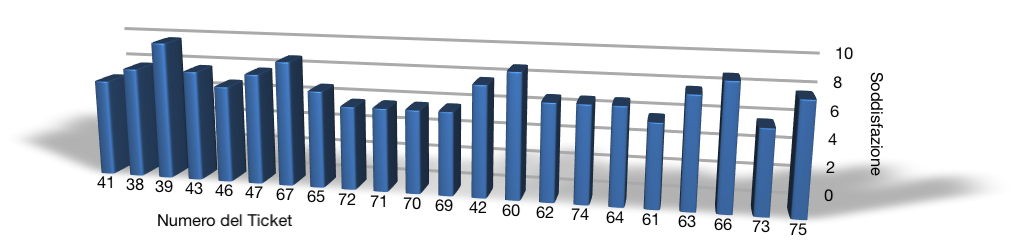
\includegraphics[height=4.1cm]{img/PQ/LavoroSvolto.png}
\caption{Feedback processo di lavoro - Lavoro svolto}
\end{figure}

\begin{figure}[htbp]
  \centering
  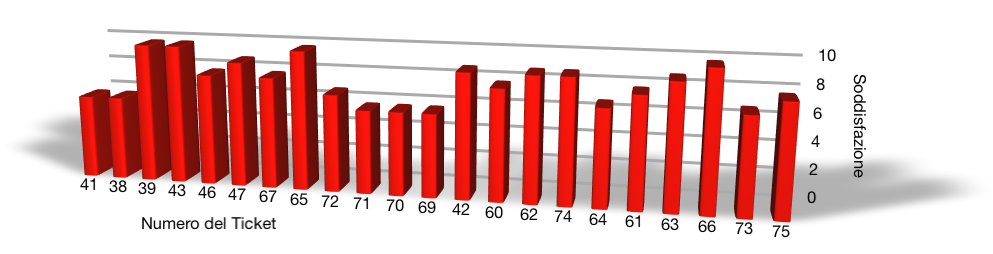
\includegraphics[height=4.1cm]{img/PQ/InterazioneConGliAltri.png}
\caption{Feedback processo di lavoro - Interazione con gli altri}
\end{figure}

\begin{figure}[htbp]
  \centering
  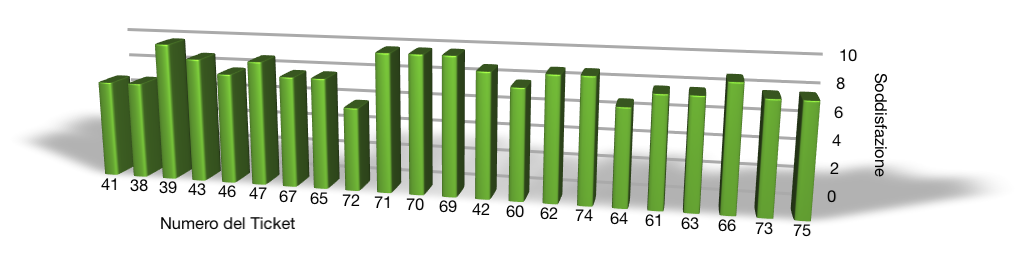
\includegraphics[height=4.1cm]{img/PQ/Strumenti.png}
\caption{Feedback processo di lavoro - Strumenti utilizzati}
\end{figure}

\begin{figure}[htbp]
  \centering
  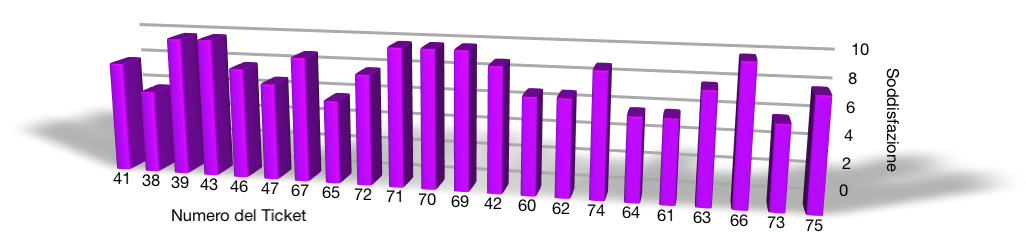
\includegraphics[height=4.1cm]{img/PQ/TempoImpiegato.png}
\caption{Feedback processo di lavoro - Tempo Impiegato}
\end{figure}

\newpage
I test di valutazione compilati in questa fase sono stati 22 e mostrano che
per:
\begin{itemize}
  \item il lavoro svolto, i membri del gruppo sono abbastanza
  soddisfatti (media voto 7.4);
  \item l'iterazione con gli altri, i membri del gruppo sono soddisfatti
  (media voto 8);
  \item gli strumenti utilizzati, i membri del gruppo
  sono molto soddisfatti (media voto 8.4);
  \item il tempo impiegato, i membri del gruppo
  sono abbastanza soddisfatti (media voto 8).\\
\end{itemize}

Questi risultati verranno confrontati con le valutazioni che si riceveranno
nella revisione RP e potranno fornire interessanti spunti su come correggere o
rafforzare il metodo di lavoro.

\end{document}

